\begin{flushright} {\tiny {\color{gray} python\_codes/fieldstone\_129/text.tex}} \end{flushright}

\lstinputlisting[language=bash,basicstyle=\small]{python_codes/fieldstone_129/keywords}

\begin{center}
\fbox{\textbf{\huge \color{teal} P}}
Codes at \url{https://github.com/cedrict/fieldstone/tree/master/python_codes/fieldstone_129}
\end{center}

%%%%%%%%%%%%%%%%%%%%%%%%%%%%%%%%%%%%%%%%%%%%%%%%%%%%%%%%%%%%%%%%%%%%%%%%%%%%%%%%%%%%%%%%%%%%%%
\par\noindent\rule{\textwidth}{0.4pt}

{\sl This stone was developed in collaboration with Taco Broerse}. \index{contributors}{T. Broerse}

\par\noindent\rule{\textwidth}{0.4pt}
%%%%%%%%%%%%%%%%%%%%%%%%%%%%%%%%%%%%%%%%%%%%%%%%%%%%%%%%%%%%%%%%%%%%%%%%%%%%%%%%%%%%%%%%%%%%%%




We start from Eq.~(12.40) in the book of Simpson (I here use my notations
and not those of the book):
\begin{eqnarray}
\dot{\bm\varepsilon}^d
&=&\frac{1}{2\mu} \frac{\partial \bm\tau}{\partial t}
+\frac{1}{2\eta} \bm\tau \nn\\
&\simeq&
\frac{1}{2\mu} \frac{\bm\tau - \bm\tau^0}{\delta t}
+\frac{1}{2\eta} \bm\tau \nn\\
&=&
\frac12 \left( \frac{1}{\mu \delta t} + \frac{1}{\eta} \right) {\bm\tau}
-\frac{1}{2\mu \delta t} \bm\tau^0\nn\\
&=&
\frac12 \frac{ \mu\delta t +\eta}{\mu \delta t \eta}  {\bm\tau}
-\frac{1}{2\mu \delta t} \bm\tau^0
\end{eqnarray}
where ${\bm \tau}^0$ is the already known/previous deviatoric stress tensor. This can be rewritten as
\begin{eqnarray}
\bm\tau 
%&=& 2\left( \frac{1}{\mu \delta t} + \frac{1}{\eta} \right)^{-1} \dot{\bm\varepsilon}^d -2
%\left( \frac{1}{\mu \delta t} + \frac{1}{\eta} \right)^{-1} \frac{1}{2\mu \delta t} \bm\tau^0 
%\nn\\
%&=& 2 \left( \frac{ \mu\delta t +\eta}{\mu \delta t \eta}   \right)^{-1} \dot{\bm\varepsilon}^d -
%2 \left( \frac{\mu\delta t + \eta}{\mu \delta t \eta} \right)^{-1} \frac{1}{2\mu \delta t} \bm\tau^0
%\nn\\
&=&
2  \frac{\mu \delta t \; \eta}{ \mu\delta t +\eta} \dot{\bm\varepsilon}^d 
+
2 \frac{\mu \delta t \; \eta}{\mu\delta t + \eta} \frac{1}{2\mu \delta t} \bm\tau^0
\nn\\
&=&
\frac{2 \mu \delta t \eta}{ \mu\delta t +\eta} \dot{\bm\varepsilon}^d 
+
\frac{ \eta}{\mu\delta t + \eta}  \bm\tau^0 \label{tau_simp1}
\end{eqnarray}

Defining the mean stress $\sigma_m$ as
\[
\sigma_m = \frac13(\sigma_{xx}+\sigma_{yy}+\sigma_{zz})
\]
then by definition of the deviatoric stress 
$\bm\tau = \bm\sigma -\sigma_m {\bm 1} $. 
Also, the viscous deformation is deviatoric so the volume changes
are only due to the elastic deformation and we have\footnote{
In the book it is written as $\sigma_m = 3K \varepsilon_v $}
\[
\sigma_m 
%= 3K \varepsilon_v 
= K {\rm tr}({\bm\varepsilon})
\]
Then
\[
\frac{\partial\sigma_m}{\partial t} 
\simeq 
\frac{\sigma_m - \sigma_m^0}{\delta t}
= K {\rm tr}(\dot{\bm\varepsilon})
\qquad
\Rightarrow
\qquad
\sigma_m \simeq K  {\rm tr}(\dot{\bm\varepsilon}) \delta t + \sigma_m^0
\]
and then
\[
\bm\tau = \bm\sigma -\sigma_m {\bm 1} 
= \bm\sigma - [K {\rm tr}(\dot{\bm\varepsilon}) \delta t + \sigma_m^0] {\bm 1}
\]
Inserting this in Eq.~\eqref{tau_simp1}
we obtain 
\begin{mdframed}[backgroundcolor=blue!5]
\begin{eqnarray}
\bm \sigma 
&=& 
K {\rm tr}(\dot{\bm\varepsilon}) \delta t {\bm 1}  +
\frac{2 \mu \eta\delta t}{ \mu\delta t +\eta} \dot{\bm\varepsilon}^d +
\frac{ \eta}{\mu\delta t + \eta}  \bm\tau^0 + \sigma_m^0 {\bm 1}
\end{eqnarray}
\end{mdframed}

We can now switch to using a vector representation of the tensors\footnote{We need to be extra careful about the strain rate vector $\dot{\vec{\varepsilon}}$ since it contains a factor 2 in front of the off diagonal tensor terms, hence the ${\bm C}$ tensor.} as it is necessary for implementation in a FEM code:
\begin{eqnarray}
{\bm \sigma} &\rightarrow& \vec{\sigma} \nn\\
{\bm \varepsilon} &\rightarrow& {\bm C} \cdot \vec{\varepsilon} \nn\\
{\bm 1} &\rightarrow& \vec{m} \nn
\end{eqnarray}
with 
\[
\vec{m}=
\left(
\begin{array}{c}
1 \\ 1 \\ 1 \\ 0 \\ 0 \\ 0
\end{array}
\right),
\qquad\quad
{\bm C}=
\left(
\begin{array}{cccccc}
1 & 0 & 0 & 0 & 0 & 0 \\
0 & 1 & 0 & 0 & 0 & 0 \\
0 & 0 & 1 & 0 & 0 & 0 \\
0 & 0 & 0 & 1/2 & 0 & 0 \\
0 & 0 & 0 & 0 & 1/2 & 0 \\
0 & 0 & 0 & 0 & 0 & 1/2 
\end{array}
\right),
\qquad
{\rm and} 
\qquad
\dot{\vec{\varepsilon}}=
\left(
\begin{array}{c}
\dot\varepsilon_{xx}\\ 
\dot\varepsilon_{yy}\\ 
\dot\varepsilon_{zz}\\ 
{\color{teal}2}\dot\varepsilon_{xy} \\ 
{\color{teal}2}\dot\varepsilon_{xz} \\ 
{\color{teal}2}\dot\varepsilon_{yz}
\end{array}
\right).
\]
%so that 
%\[
%\vec{\sigma} = K {\rm tr}(\dot{\bm\varepsilon}) \delta t \vec{m} +
%\frac{2 \mu \delta t}{ \mu\delta t +\eta} \dot{\vec{\bm\varepsilon}}^d -
%\frac{ \eta}{\mu\delta t + \eta}  \bm\tau^0 + \sigma_m^0 \vec{m}
%\]
Also, as we have seen in Eq.~\eqref{eq:el:opla1} we have
$\vec\tau = {\bm I}_d \cdot \vec\sigma$
%and $\vec\varepsilon^d = {\bm I}_d \cdot \vec\varepsilon$
with ${\bm I}_d$ the deviatoric operator:
\[
{\bm I}_d=
\left(
\begin{array}{cccccc}
\frac23 & - \frac13 & - \frac13 & 0 & 0 & 0 \\
-\frac13 & \frac23 & - \frac13  & 0 & 0 & 0\\
-\frac13& - \frac13 & \frac23  & 0 & 0 & 0\\
0&0&0& 1&0 &0  \\
0&0&0&0&1 &0\\
0&0&0&0&0& 1
\end{array}
\right)
\]
so that now
\begin{eqnarray}
\vec{\sigma} 
&=& K {\rm tr}(\dot{\bm\varepsilon}) \delta t \vec{m} +
\frac{2 \mu \eta\delta t}{ \mu\delta t +\eta} {\bm I}_d \cdot {\bm C} \cdot\dot{\vec{\bm\varepsilon}} 
+\frac{ \eta}{\mu\delta t + \eta} {\bm I}_d \cdot \bm\sigma^0 + \sigma_m^0 \vec{m} \nn\\
&=& 
\left(
\begin{array}{c}
K {\rm tr}(\dot{\bm\varepsilon}) \delta t \\
K {\rm tr}(\dot{\bm\varepsilon}) \delta t \\
K {\rm tr}(\dot{\bm\varepsilon}) \delta t \\
0 \\ 
0 \\
0
\end{array}
\right)
+
\frac{2 \mu \eta \delta t}{ \mu\delta t +\eta} 
\left(
\begin{array}{cccccc}
\frac23 & - \frac13 & - \frac13 & 0 & 0 & 0 \\
-\frac13 & \frac23 & - \frac13  & 0 & 0 & 0\\
-\frac13& - \frac13 & \frac23  & 0 & 0 & 0\\
0&0&0& 1&0 &0  \\
0&0&0&0&1 &0\\
0&0&0&0&0& 1
\end{array}
\right)
\cdot 
\left(
\begin{array}{cccccc}
1 & 0 & 0 & 0 & 0 & 0 \\
0 & 1 & 0 & 0 & 0 & 0 \\
0 & 0 & 1 & 0 & 0 & 0 \\
0 & 0 & 0 & 1/2 & 0 & 0 \\
0 & 0 & 0 & 0 & 1/2 & 0 \\
0 & 0 & 0 & 0 & 0 & 1/2 
\end{array}
\right)
\cdot
\left(
\begin{array}{c}
\dot\varepsilon_{xx}\\ 
\dot\varepsilon_{yy}\\ 
\dot\varepsilon_{zz}\\ 
{\color{teal}2}\dot\varepsilon_{xy} \\
{\color{teal}2}\dot\varepsilon_{xz} \\
{\color{teal}2}\dot\varepsilon_{yz}
\end{array}
\right) 
\nn\\
&+& 
\frac{ \eta}{\mu\delta t + \eta}
\left(
\begin{array}{cccccc}
\frac23 & - \frac13 & - \frac13 & 0 & 0 & 0 \\
-\frac13 & \frac23 & - \frac13  & 0 & 0 & 0\\
-\frac13& - \frac13 & \frac23  & 0 & 0 & 0\\
0&0&0& 1&0 &0  \\
0&0&0&0&1 &0\\
0&0&0&0&0& 1
\end{array}
\right)
\cdot
\left(
\begin{array}{c}
\sigma_{xx}^0\\ 
\sigma_{yy}^0\\ 
\sigma_{zz}^0\\ 
\sigma_{xy}^0 \\
\sigma_{xz}^0 \\
\sigma_{yz}^0
\end{array}
\right) 
+
\sigma_m^0 
\left(
\begin{array}{c}
1\\
1\\
1\\
0\\
0\\
0
\end{array}
\right) 
\nn\\
&=&
\delta t
\left(
\begin{array}{cccccc}
K & K & K & 0 & 0 & 0\\ 
K & K & K & 0 & 0 & 0\\ 
K & K & K & 0 & 0 & 0\\ 
0 & 0 & 0 & 0 & 0 & 0 \\
0 & 0 & 0 & 0 & 0 & 0 \\
0 & 0 & 0 & 0 & 0 & 0 
\end{array}
\right)
\cdot
\left(
\begin{array}{c}
\dot\varepsilon_{xx}\\ 
\dot\varepsilon_{yy}\\ 
\dot\varepsilon_{zz}\\ 
{\color{teal}2}\dot\varepsilon_{xy} \\ 
{\color{teal}2}\dot\varepsilon_{xz} \\ 
{\color{teal}2}\dot\varepsilon_{yz}
\end{array}
\right) 
+
\frac{2 \mu  \eta\delta t}{ \mu\delta t +\eta} 
\left(
\begin{array}{cccccc}
\frac23 & - \frac13 & - \frac13 & 0 & 0 & 0 \\
-\frac13 & \frac23 & - \frac13  & 0 & 0 & 0\\
-\frac13& - \frac13 & \frac23  & 0 & 0 & 0\\
0&0&0& 1/{\color{teal}2}&0 &0  \\
0&0&0&0&1/{\color{teal}2} &0\\
0&0&0&0&0& 1/{\color{teal}2}
\end{array}
\right)
\cdot
\left(
\begin{array}{c}
\dot\varepsilon_{xx}\\ 
\dot\varepsilon_{yy}\\ 
\dot\varepsilon_{zz}\\ 
{\color{teal}2}\dot\varepsilon_{xy} \\ 
{\color{teal}2}\dot\varepsilon_{xz} \\ 
{\color{teal}2}\dot\varepsilon_{yz}
\end{array}
\right) 
\nn\\
&+& 
\frac{ \eta}{\mu\delta t + \eta}
\left(
\begin{array}{cccccc}
\frac23 & - \frac13 & - \frac13 & 0 & 0 & 0 \\
-\frac13 & \frac23 & - \frac13  & 0 & 0 & 0\\
-\frac13& - \frac13 & \frac23  & 0 & 0 & 0\\
0&0&0& 1&0 &0  \\
0&0&0&0&1 &0\\
0&0&0&0&0& 1
\end{array}
\right)
\cdot
\left(
\begin{array}{c}
\sigma_{xx}^0\\ 
\sigma_{yy}^0\\ 
\sigma_{zz}^0\\ 
\sigma_{xy}^0 \\
\sigma_{xz}^0 \\
\sigma_{yz}^0
\end{array}
\right) 
+
\left(
\begin{array}{cccccc}
\frac13 & \frac13 & \frac13 & 0 & 0 & 0 \\
\frac13 & \frac13 & \frac13 & 0 & 0 & 0 \\
\frac13 & \frac13 & \frac13 & 0 & 0 & 0 \\
0 &0 &0 & 0 & 0 & 0 \\
0 &0 &0 & 0 & 0 & 0 \\
0 &0 &0 & 0 & 0 & 0 
\end{array}
\right) 
\cdot
\left(
\begin{array}{c}
\sigma_{xx}^0\\ 
\sigma_{yy}^0\\ 
\sigma_{zz}^0\\ 
\sigma_{xy}^0 \\
\sigma_{xz}^0 \\
\sigma_{yz}^0
\end{array}
\right) 
\nn\\
&=& 
\delta t
\left[
\left(
\begin{array}{cccccc}
K & K & K & 0 & 0 & 0\\ 
K & K & K & 0 & 0 & 0\\ 
K & K & K & 0 & 0 & 0\\ 
0 & 0 & 0 & 0 & 0 & 0 \\
0 & 0 & 0 & 0 & 0 & 0 \\
0 & 0 & 0 & 0 & 0 & 0 
\end{array}
\right)
+
\frac{2 \mu \eta}{ \mu\delta t +\eta} 
\left(
\begin{array}{cccccc}
\frac23 & - \frac13 & - \frac13 & 0 & 0 & 0 \\
-\frac13 & \frac23 & - \frac13  & 0 & 0 & 0\\
-\frac13& - \frac13 & \frac23  & 0 & 0 & 0\\
0&0&0& 1/{\color{teal}2}&0 &0  \\
0&0&0&0&1/{\color{teal}2} &0\\
0&0&0&0&0& 1/{\color{teal}2}
\end{array}
\right)
\right]
\cdot
\left(
\begin{array}{c}
\dot\varepsilon_{xx}\\ 
\dot\varepsilon_{yy}\\ 
\dot\varepsilon_{zz}\\ 
{\color{teal}2}\dot\varepsilon_{xy} \\ 
{\color{teal}2}\dot\varepsilon_{xz} \\ 
{\color{teal}2}\dot\varepsilon_{yz}
\end{array}
\right) 
\nn\\
&+& 
\left[
\frac{ \eta}{\mu\delta t + \eta}
\left(
\begin{array}{cccccc}
\frac23 & - \frac13 & - \frac13 & 0 & 0 & 0 \\
-\frac13 & \frac23 & - \frac13  & 0 & 0 & 0\\
-\frac13& - \frac13 & \frac23  & 0 & 0 & 0\\
0&0&0& 1&0 &0  \\
0&0&0&0&1 &0\\
0&0&0&0&0& 1
\end{array}
\right)
+
\left(
\begin{array}{cccccc}
\frac13 & \frac13 & \frac13 & 0 & 0 & 0 \\
\frac13 & \frac13 & \frac13 & 0 & 0 & 0 \\
\frac13 & \frac13 & \frac13 & 0 & 0 & 0 \\
0 &0 &0 & 0 & 0 & 0 \\
0 &0 &0 & 0 & 0 & 0 \\
0 &0 &0 & 0 & 0 & 0 
\end{array}
\right) 
\right]
\cdot
\left(
\begin{array}{c}
\sigma_{xx}^0\\ 
\sigma_{yy}^0\\ 
\sigma_{zz}^0\\ 
\sigma_{xy}^0 \\
\sigma_{xz}^0 \\
\sigma_{yz}^0
\end{array}
\right) \nn\\
&=& 
\delta t
\left(
\begin{array}{cccccc}
K + \frac{4\mu \eta/3}{\mu \delta t + \eta} &
K - \frac{2\mu \eta/3}{\mu \delta t + \eta} &
K - \frac{2\mu \eta/3}{\mu \delta t + \eta} &
0 &0 & 0 \\
K - \frac{2\mu \eta/3}{\mu \delta t + \eta} &
K + \frac{4\mu \eta/3}{\mu \delta t + \eta} &
K - \frac{2\mu \eta/3}{\mu \delta t + \eta} &
0 &0 & 0 \\
K - \frac{2\mu \eta/3}{\mu \delta t + \eta} &
K - \frac{2\mu \eta/3}{\mu \delta t + \eta} &
K + \frac{4\mu \eta/3}{\mu \delta t + \eta} &
0 &0 & 0 \\
0 & 0 & 0 & \frac{\mu \eta }{\mu \delta t + \eta} & 0 & 0 \\
0 & 0 & 0 & 0 & \frac{\mu \eta }{\mu \delta t + \eta} & 0  \\
0 & 0 & 0 & 0 & 0 & \frac{\mu \eta }{\mu \delta t + \eta} 
\end{array}
\right)
\cdot
\left(
\begin{array}{c}
\dot\varepsilon_{xx}\\ 
\dot\varepsilon_{yy}\\ 
\dot\varepsilon_{zz}\\ 
{\color{teal}2}\dot\varepsilon_{xy} \\ 
{\color{teal}2}\dot\varepsilon_{xz} \\ 
{\color{teal}2}\dot\varepsilon_{yz}
\end{array}
\right) 
\nn\\
&+&
\left(
\begin{array}{cccccc}
\frac13\frac{3\eta + \mu \delta t}{\mu\delta t+\eta} & 
\frac13\frac{\mu \delta t}{\mu\delta t+\eta} & 
\frac13\frac{\mu \delta t}{\mu\delta t+\eta} & 0 & 0 & 0\\
\frac13\frac{\mu \delta t}{\mu\delta t+\eta} & 
\frac13\frac{3\eta + \mu \delta t}{\mu\delta t+\eta} & 
\frac13\frac{\mu \delta t}{\mu\delta t+\eta} & 0 & 0 & 0\\
\frac13\frac{\mu \delta t}{\mu\delta t+\eta} & 
\frac13\frac{\mu \delta t}{\mu\delta t+\eta} & 
\frac13\frac{3\eta + \mu \delta t}{\mu\delta t+\eta} & 0 & 0 & 0\\
0 & 0 & 0 & \frac{ \eta}{\mu\delta t + \eta} & 0 & 0 \\
0 & 0 & 0 & 0 & \frac{ \eta}{\mu\delta t + \eta} & 0  \\
0 & 0 & 0 & 0 & 0 & \frac{ \eta}{\mu\delta t + \eta} 
\end{array}
\right)
\cdot
\left(
\begin{array}{c}
\sigma_{xx}^0\\ 
\sigma_{yy}^0\\ 
\sigma_{zz}^0\\ 
\sigma_{xy}^0 \\
\sigma_{xz}^0 \\
\sigma_{yz}^0
\end{array}
\right) \label{simpson3D}
\end{eqnarray}



%---------------------------------------
\subsubsection*{In Plane strain}
We start again from
\begin{eqnarray}
\bm \sigma 
&=& 
K {\rm tr}(\dot{\bm\varepsilon}) \delta t {\bm 1}  +
\frac{2 \mu \eta\delta t}{ \mu\delta t +\eta} \dot{\bm\varepsilon}^d +
\frac{ \eta}{\mu\delta t + \eta}  \bm\tau^0 + \sigma_m^0 {\bm 1}
\end{eqnarray}

In plane strain we have $\dot\varepsilon_{zz}=\dot\varepsilon_{xz}=\dot\varepsilon_{yz}=0$ and $\sigma_{xz}=\sigma_{yz}=0$ (Note that $\sigma_{zz}\ne 0$ !). Furthermore we have\footnote{Since the spring and dashpot are in series, they are under the same stress} the viscous strain rate given by:
\[
\dot{\bm\varepsilon}_v
= \frac{1}{2\eta} {\bm \tau}
= \frac{1}{2\eta} \left( {\bm \sigma} - \frac13 {\rm tr}(\bm\sigma) {\bm 1} \right)
\]
Looking at the $zz$ component yields
\[
\dot{\varepsilon}_{v,zz} = \frac{1}{2\eta} \frac13 (2\sigma_{zz}-\sigma_{xx}-\sigma_{yy})
\]
Assuming $\dot{\varepsilon}_{v,zz}=0$ (stricly speaking only the total strain  $\dot\varepsilon_{zz}=0$ but it is then logical to assume that the 
$zz$-strain rate for both mechanisms is zero simultaneously), we obtain
$\sigma_{zz}=\frac12 (\sigma_{xx}+\sigma_{yy})$.
In that sense we can discard the $\sigma_{zz}$ equation since it is 
not unknown anymore in this case.

Note that then
\[
\sigma_m 
= \frac{1}{3}(\sigma_{xx}+\sigma_{yy}+\sigma_{zz})
= \frac{1}{3}(\sigma_{xx}+\sigma_{yy}+\frac12(\sigma_{xx}+\sigma_{yy}))
= \frac{1}{2}(\sigma_{xx}+\sigma_{yy})
\]




We are left with the $\sigma_{xx}$, $\sigma_{yy}$ and $\sigma_{xy}$
equations. All we have to do is select the 1st, 2nd and 4th lines and columns of the vectors/matrices in Eq.~\eqref{simpson3D}:

\[
\left(
\begin{array}{c}
\sigma_{xx}\\ 
\sigma_{yy}\\ 
\sigma_{xy} 
\end{array}
\right)
=
\delta t
\left(
\begin{array}{ccc}
K + \frac{4\mu \eta/3}{\mu \delta t + \eta} &
K - \frac{2\mu \eta/3}{\mu \delta t + \eta} &
0 \\
K - \frac{2\mu \eta/3}{\mu \delta t + \eta} &
K + \frac{4\mu \eta/3}{\mu \delta t + \eta} &
0  \\
0 & 0 & \frac{\mu \eta }{\mu \delta t + \eta}  \\
\end{array}
\right)
\cdot
\left(
\begin{array}{c}
\dot\varepsilon_{xx}\\ 
\dot\varepsilon_{yy}\\ 
{\color{teal}2}\dot\varepsilon_{xy} 
\end{array}
\right) 
+
\left(
\begin{array}{cccccc}
\frac13\frac{3\eta + \mu \delta t}{\mu\delta t+\eta} & 
\frac13\frac{\mu \delta t}{\mu\delta t+\eta} & 
0\\
\frac13\frac{\mu \delta t}{\mu\delta t+\eta} & 
\frac13\frac{3\eta + \mu \delta t}{\mu\delta t+\eta} & 
0\\
0 & 0 & \frac{ \eta}{\mu\delta t + \eta}  
\end{array}
\right)
\cdot
\left(
\begin{array}{c}
\sigma_{xx}^0\\ 
\sigma_{yy}^0\\ 
\sigma_{xy}^0 
\end{array}
\right) 
\]
or,
\begin{mdframed}[backgroundcolor=blue!5]
\begin{equation}
\left(
\begin{array}{c}
\sigma_{xx}\\ 
\sigma_{yy}\\ 
\sigma_{xy} 
\end{array}
\right)
=
\left(
\begin{array}{ccc}
\frac{\delta t(4\mu \eta + 3K \eta+ 3K \mu\delta t)}{3(\mu \delta t + \eta)} &
\frac{\delta t(3K \eta+ 3K \mu\delta t - 2\mu \eta)}{3(\mu \delta t + \eta)} &
0 \\
\frac{\delta t(3K \eta+ 3K \mu\delta t  - 2\mu \eta)}{3(\mu \delta t + \eta)}&
\frac{\delta t(4\mu \eta + 3K \eta+ 3K \mu\delta t)}{3(\mu \delta t + \eta)} &
0  \\
0 & 0 & \frac{\mu \eta \delta t }{\mu \delta t + \eta}  \\
\end{array}
\right)
\cdot
\left(
\begin{array}{c}
\dot\varepsilon_{xx}\\ 
\dot\varepsilon_{yy}\\ 
{\color{teal}2}\dot\varepsilon_{xy} 
\end{array}
\right) 
+
\left(
\begin{array}{cccccc}
\frac13\frac{3\eta + \mu \delta t}{\mu\delta t+\eta} & 
\frac13\frac{\mu \delta t}{\mu\delta t+\eta} & 
0\\
\frac13\frac{\mu \delta t}{\mu\delta t+\eta} & 
\frac13\frac{3\eta + \mu \delta t}{\mu\delta t+\eta} & 
0\\
0 & 0 & \frac{ \eta}{\mu\delta t + \eta}  
\end{array}
\right)
\cdot
\left(
\begin{array}{c}
\sigma_{xx}^0\\ 
\sigma_{yy}^0\\ 
\sigma_{xy}^0 
\end{array}
\right) 
\label{eq_129_2D}
\end{equation}
\end{mdframed}

In order to compare this with the book's equations, I rewrite the above equation with the 
book's notations ($\mu \rightarrow G$, $\eta\rightarrow \mu$):
\begin{eqnarray}
\left(
\begin{array}{c}
\sigma_{xx}\\ 
\sigma_{yy}\\ 
\sigma_{xy} 
\end{array}
\right)
=
\underbrace{
\left(
\begin{array}{ccc}
\frac{\delta t(4G \mu + 3K \mu+ 3K G\delta t)}{3(G \delta t + \mu)} &
\frac{\delta t(3K \mu+ 3K G\delta t - 2G \mu)}{3(G \delta t + \mu)} &
0 \\
\frac{\delta t(3K \mu+ 3K G\delta t  - 2G \mu)}{3(G \delta t + \mu)}&
\frac{\delta t(4G \mu + 3K \mu+ 3K G\delta t)}{3(G \delta t + \mu)} &
0  \\
0 & 0 & \frac{G \mu \delta t }{G \delta t + \mu}  \\
\end{array}
\right)
}_{\tilde{\bm D}}
\!
\cdot\!
\left(
\begin{array}{c}
\dot\varepsilon_{xx}\\ 
\dot\varepsilon_{yy}\\ 
{\color{teal}2}\dot\varepsilon_{xy} 
\end{array}
\right) 
+
\underbrace{
\left(
\begin{array}{cccccc}
\frac{3\mu + G \delta t}{3(G\delta t+\mu)} & 
\frac{G \delta t}{3(G\delta t+\mu)} & 
0\\
\frac{G \delta t}{3(G\delta t+\mu)} & 
\frac{3\mu + G \delta t}{3(G\delta t+\mu)} & 
0\\
0 & 0 & \frac{ \mu}{G\delta t + \eta}  
\end{array}
\right)
}_{\tilde{\bm D}_s}
\!\cdot\!
\left(
\begin{array}{c}
\sigma_{xx}^0\\ 
\sigma_{yy}^0\\ 
\sigma_{xy}^0 
\end{array}
\right) 
\nonumber
\end{eqnarray}



\begin{center}
\fbox{
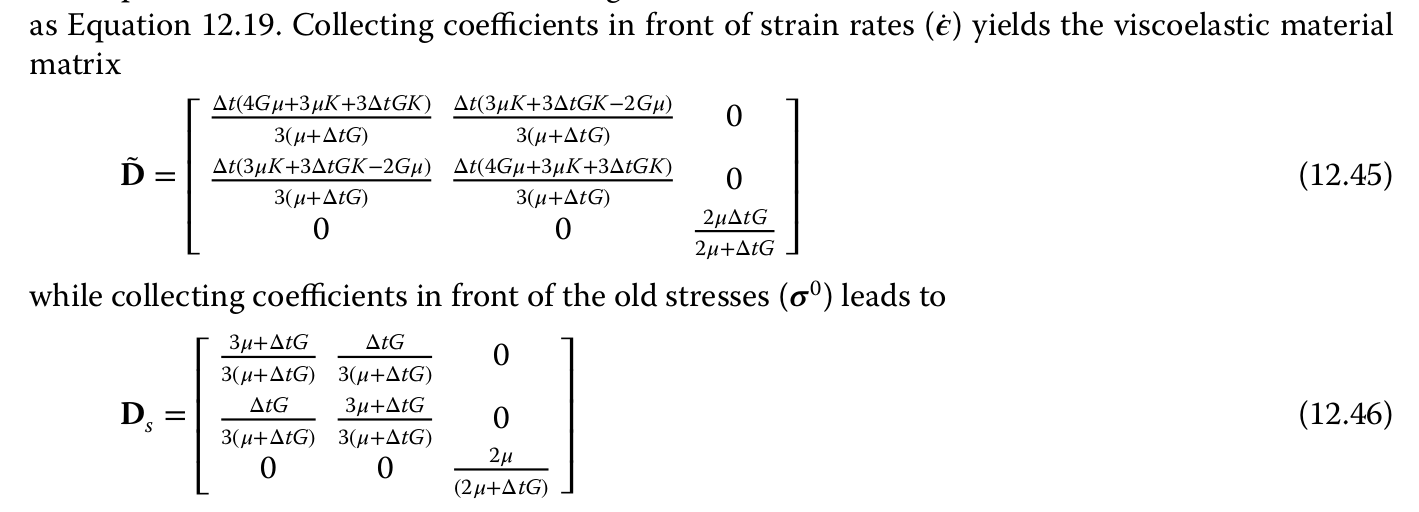
\includegraphics[width=17cm]{python_codes/fieldstone_129/images/simpson_1}}\\
{\captionfont Taken from the book.}
\end{center}

A few remarks:
\begin{itemize}
\item 
Good news, I agree with the book's equations except for the (3,3)
term which in my opinion is missing a factor 2 in front of 
the $\Delta t G$ of the denominator.
I will need an analytical benchmark to sort this out.
\item 
Also I obtain  $\vec\sigma= \tilde{\bm D} \cdot \dot{\vec{\varepsilon}} + {\bm D}_s \cdot \vec{\sigma}^0$ which is coherent with Eq.~(12.19) of the book but the book has a minus sign in front of ${\bm D}_s$ on page 188.
\item 
In any case the book is missing a discussion about the 'disappearance' of $\sigma_{yy}$ after Eq.~(12.33).
Also Eq.~(12.39) should probably showcase a factor 2 in front of
the $xz$ term.
\item The time derivative in Eq.~(12.40) is in fact the  co-rotational (Jaumann) time derivative of the deviatoric stress tensor. What is presented here is a simplification, which is ok because a Lagrangian approach is taken?
\end{itemize}

%----------------------------------------------
\subsubsection*{Using an effective viscosity}

Let us recall the following matrices
\[
{\bm \Lambda}=
\left(
\begin{array}{cccccc}
2 & 0 & 0 & 0 & 0 & 0 \\
0 & 2 & 0 & 0 & 0 & 0 \\
0 & 0 & 2 & 0 & 0 & 0 \\
0 & 0 & 0 & 1 & 0 & 0 \\
0 & 0 & 0 & 0 & 1 & 0 \\
0 & 0 & 0 & 0 & 0 & 1 
\end{array}
\right)
\qquad
{\bm \Lambda}^d
=
\left(
\begin{array}{cccccc}
\frac43 & - \frac23 & - \frac23 & 0 & 0 & 0 \\
-\frac23 & \frac43 & - \frac23  & 0 & 0 & 0\\
-\frac23& - \frac23 & \frac43  & 0 & 0 & 0\\
0&0&0& 1&0 &0  \\
0&0&0&0&1 &0\\
0&0&0&0&0& 1
\end{array}
\right)
\]
\[
\tilde{\bm \Lambda}^d
=
\left(
\begin{array}{cccccc}
\frac23 & - \frac13 & - \frac13 & 0 & 0 & 0 \\
-\frac13 & \frac23 & - \frac13  & 0 & 0 & 0\\
-\frac13& - \frac13 & \frac23  & 0 & 0 & 0\\
0&0&0& 1&0 &0  \\
0&0&0&0&1 &0\\
0&0&0&0&0& 1
\end{array}
\right)
\qquad
{\bm \Xi}=
\left(
\begin{array}{cccccc}
1 & 1 & 1 & 0 & 0 & 0\\ 
1 & 1 & 1 & 0 & 0 & 0\\ 
1 & 1 & 1 & 0 & 0 & 0\\ 
0 & 0 & 0 & 0 & 0 & 0 \\
0 & 0 & 0 & 0 & 0 & 0 \\
0 & 0 & 0 & 0 & 0 & 0 
\end{array}
\right)
\]

It is common to find in the literature the so-called effective 
viscosity $\eta_{eff}$ defined as 
\[
\eta_{eff}
=\frac{\eta \delta t}{\delta t + \eta/\mu}
=\frac{\eta}{1 + t_M/\delta t}
=\frac{\mu\eta \delta t}{\mu \delta t + \eta}
\]
and 
\[
\eta_{eff}' = \frac{\eta_{eff}}{\mu\delta t}
\]
Then 
\begin{eqnarray}
\bm \sigma 
&=& 
K {\rm tr}(\dot{\bm\varepsilon}) \delta t {\bm 1}  +
2\eta_{eff} \dot{\bm\varepsilon}^d +
\frac{ \eta_{eff}}{\mu\delta t}  \bm\tau^0 + \sigma_m^0 {\bm 1}
\end{eqnarray}



\begin{eqnarray}
\vec{\sigma} 
&=& K {\rm tr}(\dot{\bm\varepsilon}) \delta t \vec{m} +
2\eta_{eff} {\bm I}_d \cdot {\bm C} \cdot\dot{\vec{\bm\varepsilon}} 
+\frac{\eta_{eff}}{\mu\delta t} {\bm I}_d \cdot \bm\sigma^0 + \sigma_m^0 \vec{m} \nn\\
&=& 
\left(
\begin{array}{c}
K {\rm tr}(\dot{\bm\varepsilon}) \delta t \\
K {\rm tr}(\dot{\bm\varepsilon}) \delta t \\
K {\rm tr}(\dot{\bm\varepsilon}) \delta t \\
0 \\ 
0 \\
0
\end{array}
\right)
+
2\eta_{eff}
\left(
\begin{array}{cccccc}
\frac23 & - \frac13 & - \frac13 & 0 & 0 & 0 \\
-\frac13 & \frac23 & - \frac13  & 0 & 0 & 0\\
-\frac13& - \frac13 & \frac23  & 0 & 0 & 0\\
0&0&0& 1&0 &0  \\
0&0&0&0&1 &0\\
0&0&0&0&0& 1
\end{array}
\right)
\cdot 
\left(
\begin{array}{cccccc}
1 & 0 & 0 & 0 & 0 & 0 \\
0 & 1 & 0 & 0 & 0 & 0 \\
0 & 0 & 1 & 0 & 0 & 0 \\
0 & 0 & 0 & 1/2 & 0 & 0 \\
0 & 0 & 0 & 0 & 1/2 & 0 \\
0 & 0 & 0 & 0 & 0 & 1/2 
\end{array}
\right)
\cdot
\left(
\begin{array}{c}
\dot\varepsilon_{xx}\\ 
\dot\varepsilon_{yy}\\ 
\dot\varepsilon_{zz}\\ 
{\color{teal}2}\dot\varepsilon_{xy} \\
{\color{teal}2}\dot\varepsilon_{xz} \\
{\color{teal}2}\dot\varepsilon_{yz}
\end{array}
\right) 
\nn\\
&+& 
\frac{\eta_{eff}}{\mu\delta t}
\left(
\begin{array}{cccccc}
\frac23 & - \frac13 & - \frac13 & 0 & 0 & 0 \\
-\frac13 & \frac23 & - \frac13  & 0 & 0 & 0\\
-\frac13& - \frac13 & \frac23  & 0 & 0 & 0\\
0&0&0& 1&0 &0  \\
0&0&0&0&1 &0\\
0&0&0&0&0& 1
\end{array}
\right)
\cdot
\left(
\begin{array}{c}
\sigma_{xx}^0\\ 
\sigma_{yy}^0\\ 
\sigma_{zz}^0\\ 
\sigma_{xy}^0 \\
\sigma_{xz}^0 \\
\sigma_{yz}^0
\end{array}
\right) 
+
\sigma_m^0 
\left(
\begin{array}{c}
1\\
1\\
1\\
0\\
0\\
0
\end{array}
\right) 
\nn\\
&=&
\delta t
\left(
\begin{array}{cccccc}
K & K & K & 0 & 0 & 0\\ 
K & K & K & 0 & 0 & 0\\ 
K & K & K & 0 & 0 & 0\\ 
0 & 0 & 0 & 0 & 0 & 0 \\
0 & 0 & 0 & 0 & 0 & 0 \\
0 & 0 & 0 & 0 & 0 & 0 
\end{array}
\right)
\cdot
\left(
\begin{array}{c}
\dot\varepsilon_{xx}\\ 
\dot\varepsilon_{yy}\\ 
\dot\varepsilon_{zz}\\ 
{\color{teal}2}\dot\varepsilon_{xy} \\ 
{\color{teal}2}\dot\varepsilon_{xz} \\ 
{\color{teal}2}\dot\varepsilon_{yz}
\end{array}
\right) 
+
2\eta_{eff}
\left(
\begin{array}{cccccc}
\frac23 & - \frac13 & - \frac13 & 0 & 0 & 0 \\
-\frac13 & \frac23 & - \frac13  & 0 & 0 & 0\\
-\frac13& - \frac13 & \frac23  & 0 & 0 & 0\\
0&0&0& 1/{\color{teal}2}&0 &0  \\
0&0&0&0&1/{\color{teal}2} &0\\
0&0&0&0&0& 1/{\color{teal}2}
\end{array}
\right)
\cdot
\left(
\begin{array}{c}
\dot\varepsilon_{xx}\\ 
\dot\varepsilon_{yy}\\ 
\dot\varepsilon_{zz}\\ 
{\color{teal}2}\dot\varepsilon_{xy} \\ 
{\color{teal}2}\dot\varepsilon_{xz} \\ 
{\color{teal}2}\dot\varepsilon_{yz}
\end{array}
\right) 
\nn\\
&+& 
\frac{\eta_{eff}}{\mu\delta t}
\left(
\begin{array}{cccccc}
\frac23 & - \frac13 & - \frac13 & 0 & 0 & 0 \\
-\frac13 & \frac23 & - \frac13  & 0 & 0 & 0\\
-\frac13& - \frac13 & \frac23  & 0 & 0 & 0\\
0&0&0& 1&0 &0  \\
0&0&0&0&1 &0\\
0&0&0&0&0& 1
\end{array}
\right)
\cdot
\left(
\begin{array}{c}
\sigma_{xx}^0\\ 
\sigma_{yy}^0\\ 
\sigma_{zz}^0\\ 
\sigma_{xy}^0 \\
\sigma_{xz}^0 \\
\sigma_{yz}^0
\end{array}
\right) 
+
\left(
\begin{array}{cccccc}
\frac13 & \frac13 & \frac13 & 0 & 0 & 0 \\
\frac13 & \frac13 & \frac13 & 0 & 0 & 0 \\
\frac13 & \frac13 & \frac13 & 0 & 0 & 0 \\
0 &0 &0 & 0 & 0 & 0 \\
0 &0 &0 & 0 & 0 & 0 \\
0 &0 &0 & 0 & 0 & 0 
\end{array}
\right) 
\cdot
\left(
\begin{array}{c}
\sigma_{xx}^0\\ 
\sigma_{yy}^0\\ 
\sigma_{zz}^0\\ 
\sigma_{xy}^0 \\
\sigma_{xz}^0 \\
\sigma_{yz}^0
\end{array}
\right) 
\nn\\
&=& 
\left[
K \delta t {\bm \Xi}
+
\eta_{eff} {\bm \Lambda}^d
\right]
\cdot
\left(
\begin{array}{c}
\dot\varepsilon_{xx}\\ 
\dot\varepsilon_{yy}\\ 
\dot\varepsilon_{zz}\\ 
{\color{teal}2}\dot\varepsilon_{xy} \\ 
{\color{teal}2}\dot\varepsilon_{xz} \\ 
{\color{teal}2}\dot\varepsilon_{yz}
\end{array}
\right) 
+ 
\left[
\frac{\eta_{eff}}{\mu\delta t}
\tilde{\bm\Lambda}^d
+
\frac13 {\bm \Xi}
\right]
\cdot
\left(
\begin{array}{c}
\sigma_{xx}^0\\ 
\sigma_{yy}^0\\ 
\sigma_{zz}^0\\ 
\sigma_{xy}^0 \\
\sigma_{xz}^0 \\
\sigma_{yz}^0
\end{array}
\right) 
\label{simpson3D_b}
\end{eqnarray}







\begin{mdframed}[backgroundcolor=blue!5]
\[
\vec\sigma = 
\left(
K \delta t {\bm \Xi}
+
\eta_{eff} {\bm \Lambda}^d
\right)
\cdot
\dot{\vec{\varepsilon}}
+
\left[
\frac{\eta_{eff}}{\mu\delta t}
\tilde{\bm\Lambda}^d
+
\frac13 {\bm \Xi}
\right]
\cdot
\vec\sigma_0
\]
\end{mdframed}

We see that this yields much more compact notations
than the section above.



%----------------------------------------------
\paragraph{End member: infinite viscosity}
In this case the Maxwell time $t_M=\eta/mu$ is very large.
We have $\eta/\mu >> \delta t$ so that $\eta_{eff} 
\rightarrow \mu \delta t$. This makes sense, infinite 
viscosity means that the dashpot behaves as a rigid block 
and its viscosity will not play a role in the deformation
and it'll propagate the stress to the spring.

Then 
\[
\frac{\eta_{eff}}{\mu \delta t} \tilde{\bm\Lambda}^d + 
\frac13 {\bm\Xi} 
\rightarrow
\tilde{\bm\Lambda}^d + 
\frac13 {\bm\Xi} 
=
{\bm I}
\]

Then
\begin{eqnarray}
\vec{\sigma}
&=&
\left(
K \delta t {\bm \Xi}
+
\mu \delta t {\bm \Lambda}^d
\right)
\cdot
\dot{\vec{\varepsilon}}
+
\vec{\sigma}_0 \nn\\
&=& 
\delta t (K  {\bm \Xi}
+ \mu  {\bm \Lambda}^d) \cdot 
\dot{\vec{\varepsilon}}
+
\vec{\sigma}_0 
\end{eqnarray}
or,
\[
\frac{\vec\sigma - \vec\sigma_0}{\delta t}
=(
K  {\bm \Xi}
+ \mu  {\bm \Lambda}^d)
\cdot \dot{\vec{\varepsilon}}
\]
which is a discretised form of the time derivative of Eq.~(XYZ). It all makes sense, we recover a purely 
elastic formulation!


%----------------------------------------------
\paragraph{End member: infinite shear modulus}
In this case the Maxwell time is very small and the effective
viscosity tends to the real viscosity and also  
\[
\frac{\eta_{eff}}{\mu \delta t} 
\rightarrow 
\frac{\eta}{\mu \delta t} 
\rightarrow 0
\]

Then

\begin{eqnarray}
\vec{\sigma}
&=&
\left(
K \delta t {\bm \Xi}
+
\eta {\bm \Lambda}^d
\right)
\cdot
\dot{\vec{\varepsilon}}
+
\vec{\sigma}_0 \nn\\
&=& 
\end{eqnarray}

This looks like the standard penalty formulation, except for 
the $\vec{\sigma}_0$ term...?

This also probably means that reduced integration can/should be done ?

%------------------------------------------------------------------------------
\subsection*{Implementation details}

Following chapter 12 of Guy Simpson's book\footnote{I have slightly changed the notations.} \cite{simp17} 
or following the derivations above we have Eq.~\eqref{eq_129_2D}
which I here recall:

\[
\left(
\begin{array}{c}
\sigma_{xx}\\ 
\sigma_{yy}\\ 
\sigma_{xy} 
\end{array}
\right)
=
\left(
\begin{array}{ccc}
\frac{\delta t(4\mu \eta + 3K \eta+ 3K \mu\delta t)}{3(\mu \delta t + \eta)} &
\frac{\delta t(3K \eta+ 3K \mu\delta t - 2\mu \eta)}{3(\mu \delta t + \eta)} &
0 \\
\frac{\delta t(3K \eta+ 3K \mu\delta t  - 2\mu \eta)}{3(\mu \delta t + \eta)}&
\frac{\delta t(4\mu \eta + 3K \eta+ 3K \mu\delta t)}{3(\mu \delta t + \eta)} &
0  \\
0 & 0 & \frac{\mu \eta \delta t }{\mu \delta t + \eta}  \\
\end{array}
\right)
\cdot
\left(
\begin{array}{c}
\dot\varepsilon_{xx}\\ 
\dot\varepsilon_{yy}\\ 
{\color{teal}2}\dot\varepsilon_{xy} 
\end{array}
\right) 
+
\left(
\begin{array}{cccccc}
\frac13\frac{3\eta + \mu \delta t}{\mu\delta t+\eta} & 
\frac13\frac{\mu \delta t}{\mu\delta t+\eta} & 
0\\
\frac13\frac{\mu \delta t}{\mu\delta t+\eta} & 
\frac13\frac{3\eta + \mu \delta t}{\mu\delta t+\eta} & 
0\\
0 & 0 & \frac{ \eta}{\mu\delta t + \eta}  
\end{array}
\right)
\cdot
\left(
\begin{array}{c}
\sigma_{xx}^0\\ 
\sigma_{yy}^0\\ 
\sigma_{xy}^0 
\end{array}
\right) 
\]
or, 
\[
\vec{\sigma} = \tilde{\bm D}\cdot \vec{\dot{\varepsilon}} +
{\bm D}_s \cdot \vec{\sigma}_0 
\]
Note the green '2' in the equation above: in Simpson's book it is in the
lower right term of the matrix. Also, Simpson uses $\mu$ for the viscosity
while we here use $\eta$. 

We see that pressure is not a degree of freedom so the finite element
formulation and discretisation will not yield a saddle point problem, 
which is a good thing in terms of complexity and solving procedure.

In the end the following weak form is obtained:
\[
\int {\bm B}^T \cdot \tilde{\bm D} \cdot {\bm B} dV \cdot \vec{\cal V} 
= \int \vec{\bN} \rho \vec{g} dV -\int {\bm B}^T \cdot {\bm D}_s \cdot \vec{\sigma}_0 dV
\]

We need to keep track of the stress $\vec{\sigma}_0$ and 
we do so directly at the quadrature points.
The strain rate vector is recomputed at every time step but it is also 
directly stored on the quadrature points.

The current stress vector $\vec{\sigma}$ is also on the quadrature points and
is computed by means of the equation above.

In the end we declare the following arrays:
\begin{lstlisting}
nqperdim=3
nq=nel*nqperdim**ndim # total number of quadrature points
stress0_vector    = np.zeros((3,nq),dtype=np.float64) # stress vector memory
stress_vector     = np.zeros((3,nq),dtype=np.float64) # stress vector 
strainrate_vector = np.zeros((3,nq),dtype=np.float64) # strain rate vector
\end{lstlisting}

The code relies on quadratic elements ($Q_2$).
Each element is assigned a 'phase' (a material) and 
each material can have different values of $\mu, \eta, \nu, K, E$.

As is common when modelling elasto-viscous materials
we define an effective viscosity:
\[
\eta_{eff} 
= \frac{\eta \delta t}{\delta t + \eta/\mu} 
= \frac{\eta }{1 + \eta/(\mu \delta t)} 
\]
Note that if $\mu\rightarrow \infty$ (or rather $\mu \delta t >> \eta$) 
then $\eta_{eff} \rightarrow \eta$. 





The 'stress memory' rhs is computed as follows:
\begin{lstlisting}
f_el-=b_mat.T.dot(stress_vector[:,counterq])*weightq*jcob
\end{lstlisting}



The mesh deforms with the material flow (Lagrangian approach)
and this is simply implemented as follows 

\begin{lstlisting}
xV[:]+=u[:]*dt
yV[:]+=v[:]*dt
\end{lstlisting}

The mean stress can also be computed and visualised:
\[
\sigma_m 
= \frac{1}{3}(\sigma_{xx}+\sigma_{yy}+\sigma_{zz})
= \frac{1}{3}(\sigma_{xx}+\sigma_{yy}+\frac12(\sigma_{xx}+\sigma_{yy}))
= \frac{1}{2}(\sigma_{xx}+\sigma_{yy})
\]

The matrix $\tilde{\bm D}$ is implemented as follows:

\begin{lstlisting}
di=dt*(3*eta[iel]*K[iel]+3*dt*mu[iel]*K[iel]+4*mu[iel]*eta[iel])
od=dt*(-2*mu[iel]*eta[iel]+3*eta[iel]*K[iel]+3*dt*mu[iel]*K[iel])
d=3*(eta[iel]+dt*mu[iel])
ed=eta[iel]*dt*mu[iel]/(eta[iel]+dt*mu[iel])
Dee = np.array([[di/d, od/d,  0],\
                [od/d, di/d,  0],\
                [0,       0, ed]],dtype=np.float64)
\end{lstlisting}
while the matrix ${\bm D}_s$ is implemented as follows
\begin{lstlisting}
di=3*eta[iel]+dt*mu[iel]
od=dt*mu[iel] 
ed=eta[iel]/(eta[iel]+dt*mu[iel]) 
Dees = np.array([[di/d, od/d,  0],\
                 [od/d, di/d,  0],\
                 [0,       0, ed]],dtype=np.float64)
\end{lstlisting}

In the case of a power-law viscous rheology, we have $\dot{\varepsilon}=A \tau^n$.
If we now write $\tau=2 \eta_{eff} \dot\varepsilon$, or
\[
\eta_{eff} = \frac12 \frac{\tau}{\dot\varepsilon} = \frac12 \frac{\tau}{A \tau^n} = \frac12 A^{-1} \tau^{1-n}
\]


Are there visco-elastic benchmarks ? bepo10 ?




\newpage
%------------------------------------------------------------------------------
\subsection*{Folding (experiment=1)}

Boundary conditions are free slip on the left, right and bottom boundaries, while
a horizontal velocity of $\SI{5}{\mm\per\year}$ is prescribed on the right 
boundary\footnote{The vertical component of the velocity 
on the right wall is not clear, but looking at the figure we see that 
the thickening is the same on the left and right, so that the
vertical velocity on the right is unconstrained.}.

In the book, the time step is fixed to 
\[
\delta t = 0.01/edot = 0.01*Lx/u_{bc} = 0.01*4/5e-3 = \SI{0.8}{\year}
\]

\begin{center}
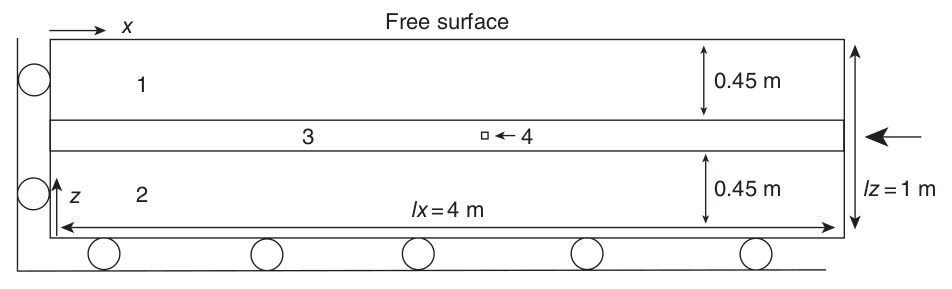
\includegraphics[width=13cm]{python_codes/fieldstone_129/images/simpson1}\\
{\captionfont  
Numbers indicate the lithological unit (termed the ``phase'' in the Matlab script). 
The folding experiment was
performed with a viscoelastic material where the central layer (i.e., phases 3 and 4) 
has a shear viscosity ($\eta=\SI{1e20}{\pascal\second}$) that
is 100 times greater than that of the surrounding matrix ($\SI{1e18}{\pascal\second}$). 
Other parameters are as follows: 
density = $\SI{2700}{\kg\per\cubic\meter}$ , 
gravity = $\SI{9.8}{\meter\per\square\second}$, 
Young's modulus = $\SI{1e11}{\pascal}$, 
Poisson’s ratio = 0.3 (all considered uniform throughout),
and a 40x40 elements.}
\end{center}

The position of the nodes on the interface between the layer and the matrix is 
perturbed with a random signal:
\begin{lstlisting}
for i in range(0,NV):
    if abs(yV[i]-0.45)/Ly<eps:
       yV[i]+=hy*0.05*random.uniform(-1,1)
    if abs(yV[i]-0.55)/Ly<eps:
       yV[i]+=hy*0.05*random.uniform(-1,1)
\end{lstlisting}


\begin{center}
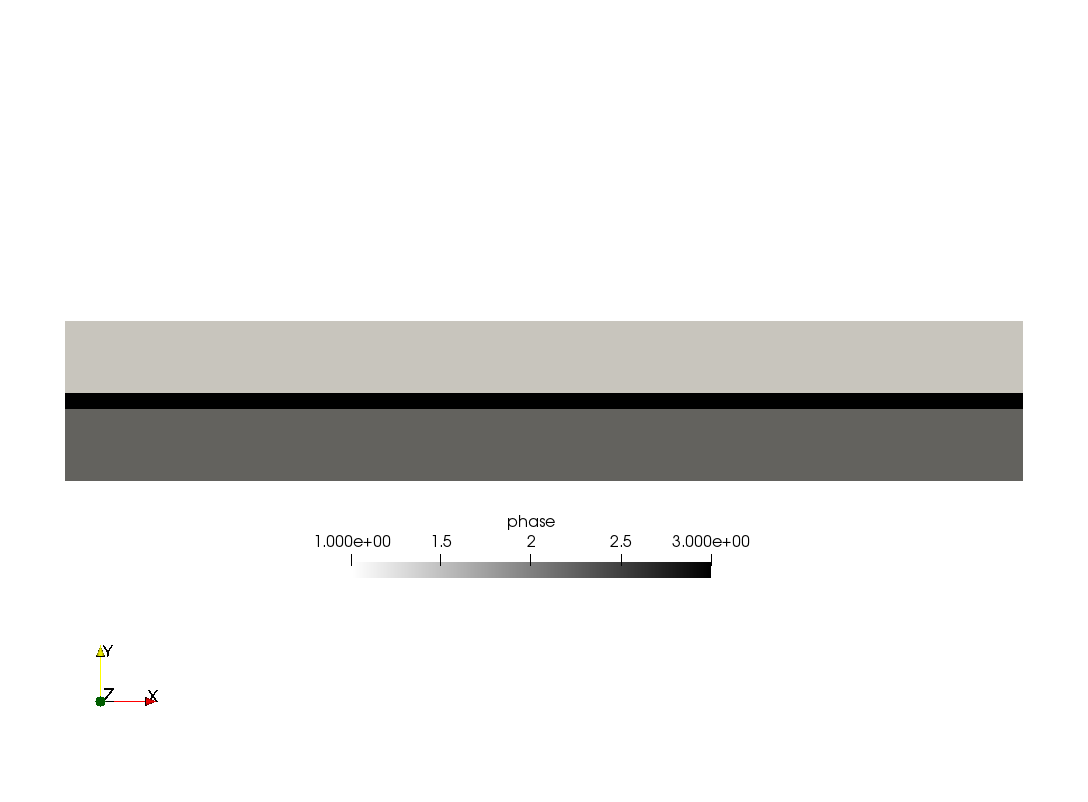
\includegraphics[width=5.7cm]{python_codes/fieldstone_129/results/experiment1/phase}
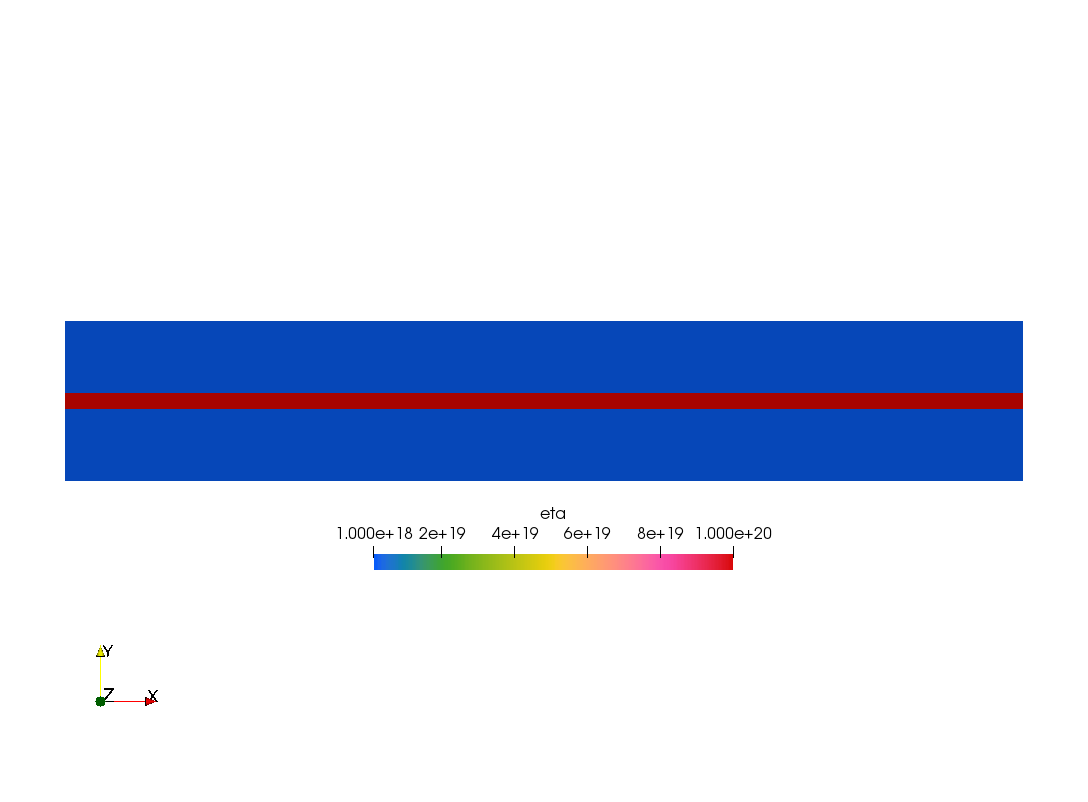
\includegraphics[width=5.7cm]{python_codes/fieldstone_129/results/experiment1/eta}
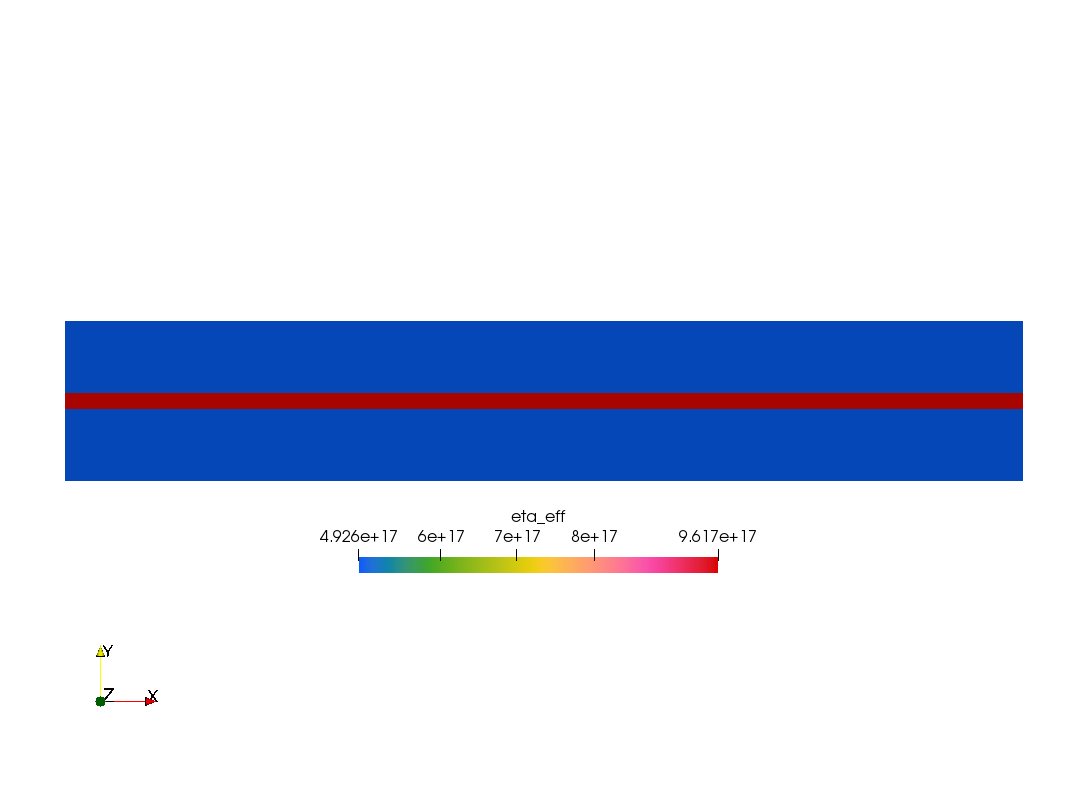
\includegraphics[width=5.7cm]{python_codes/fieldstone_129/results/experiment1/etaeff}\\
{\captionfont Initial setup of the experiment.}
\end{center} 

\begin{verbatim}
viscosity eta    = [1.e+18 1.e+18 1.e+20]
Young modulus E  = [1.e+11 1.e+11 1.e+11]
shear modulus mu = [3.84615385e+10 3.84615385e+10 3.84615385e+10]
bulk modulus K   = [8.33333333e+10 8.33333333e+10 8.33333333e+10]
poisson ratio nu = [0.3 0.3 0.3]
\end{verbatim}


\begin{center}
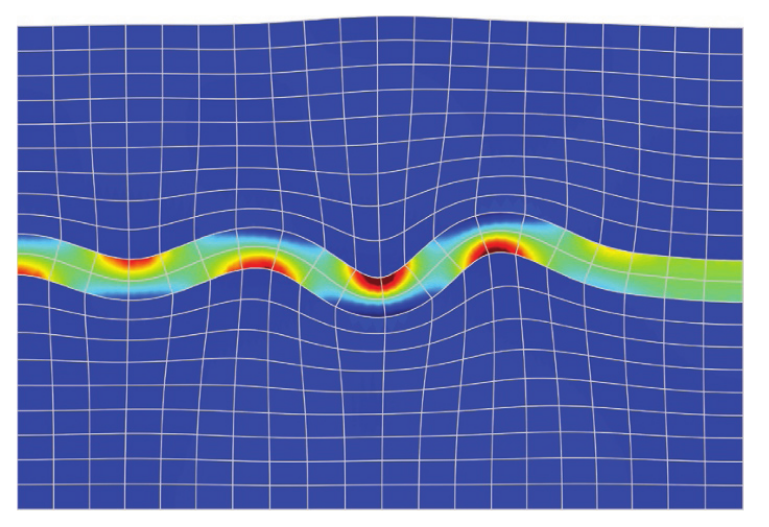
\includegraphics[width=10cm]{python_codes/fieldstone_129/images/simpson2}\\
{\captionfont 
Folding in a layered viscoelastic material after 40\% shortening. The central 
layer has a viscosity 100 higher than the surrounding matrix. The shaded colors 
represent mean stress, while the grid shows finite deformation 
(which is not the computational mesh). Unfortunately no color legend.}
\end{center}

what about pre-stress, initial compaction?

Remark:
- p191, viscosity values in 1) are wrong ? different?



\begin{center}
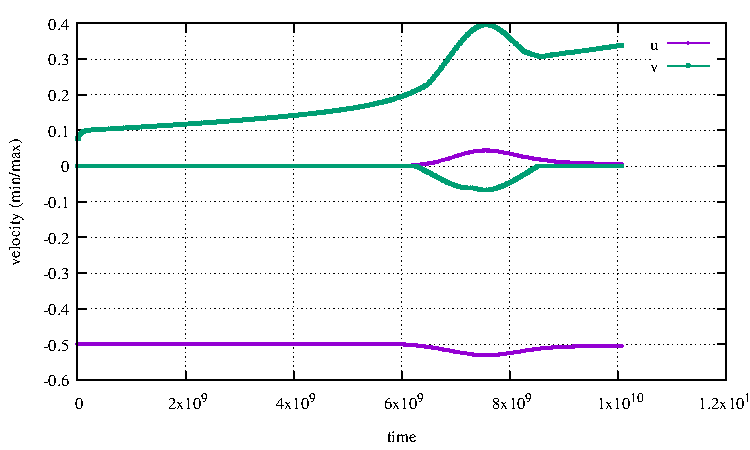
\includegraphics[width=5.7cm]{python_codes/fieldstone_129/results/experiment1/stats_velocity}
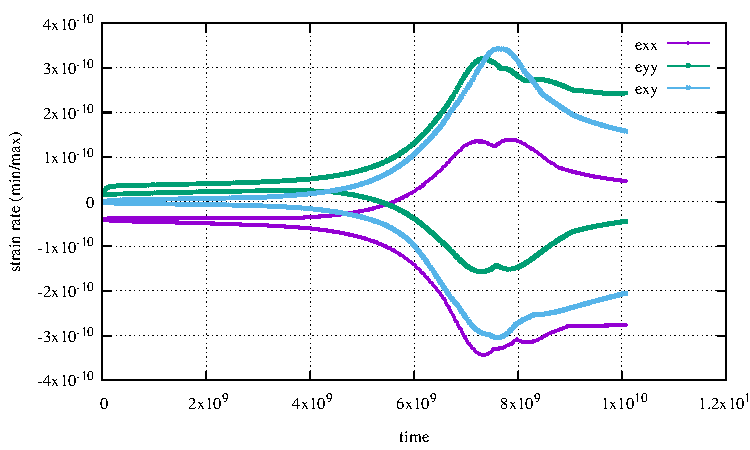
\includegraphics[width=5.7cm]{python_codes/fieldstone_129/results/experiment1/stats_strainrate}
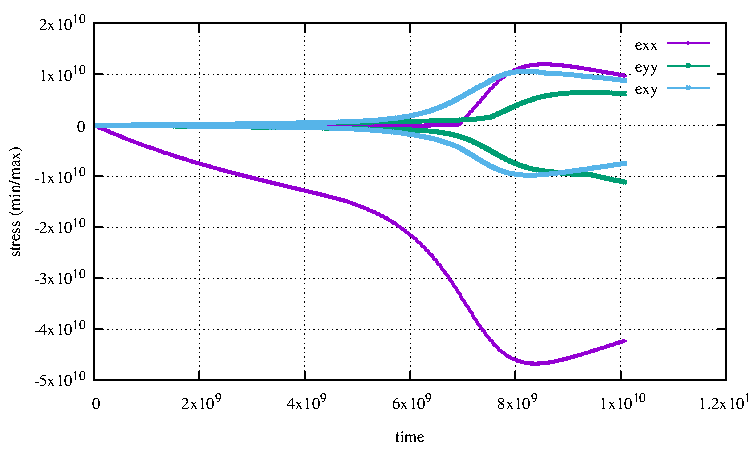
\includegraphics[width=5.7cm]{python_codes/fieldstone_129/results/experiment1/stats_stress}\\
{\captionfont a}
\end{center} 


\begin{center}
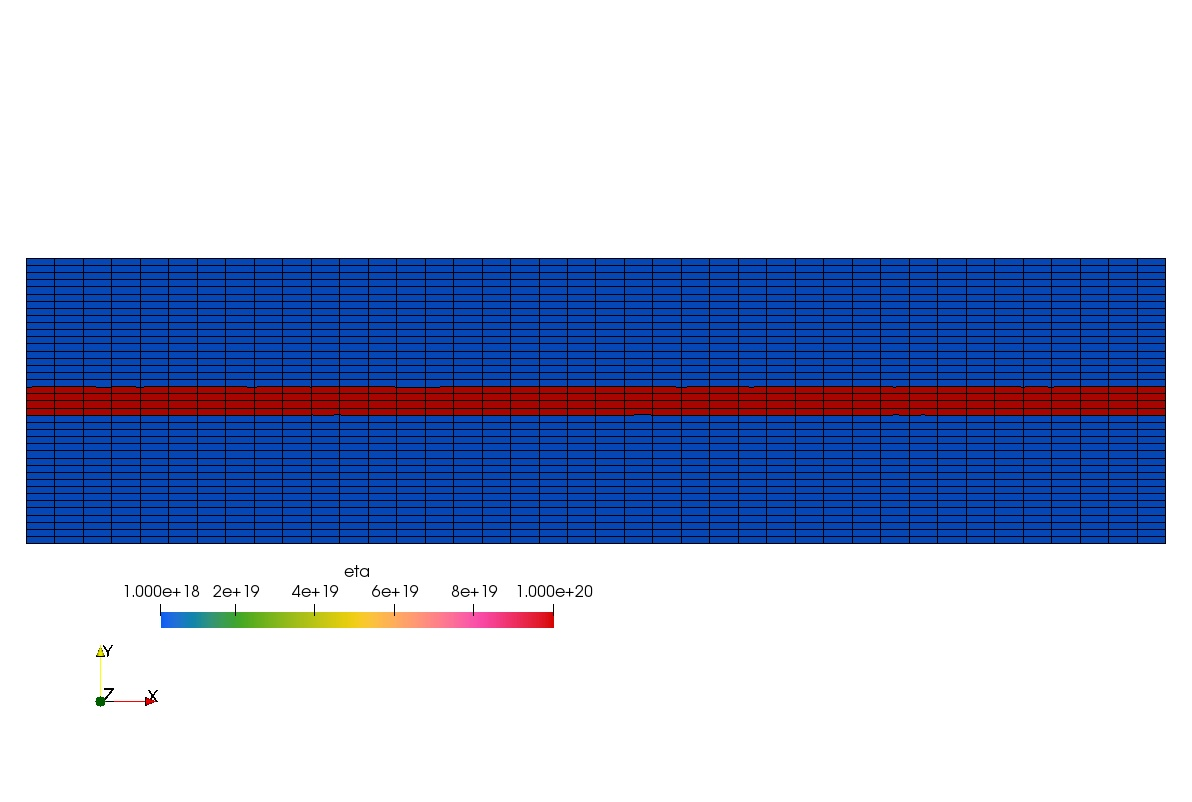
\includegraphics[width=3.4cm]{python_codes/fieldstone_129/results/experiment1/eta0000}
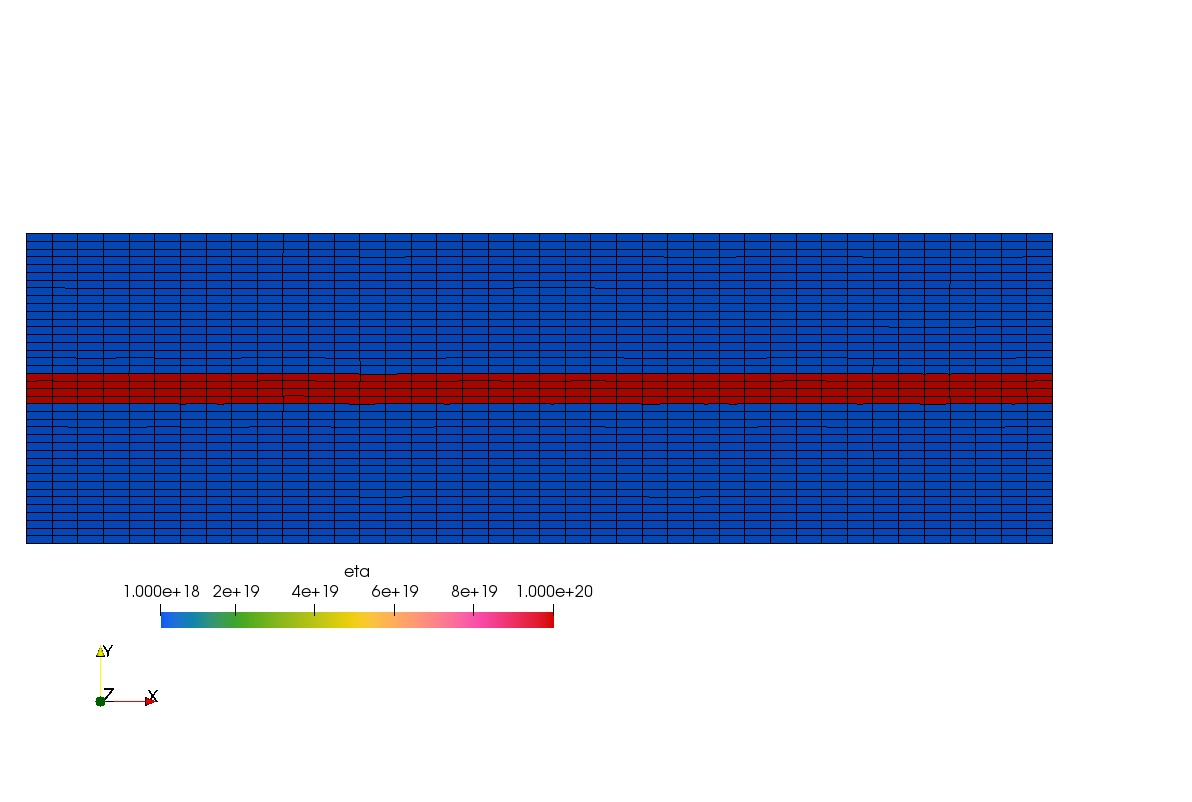
\includegraphics[width=3.4cm]{python_codes/fieldstone_129/results/experiment1/eta0099}
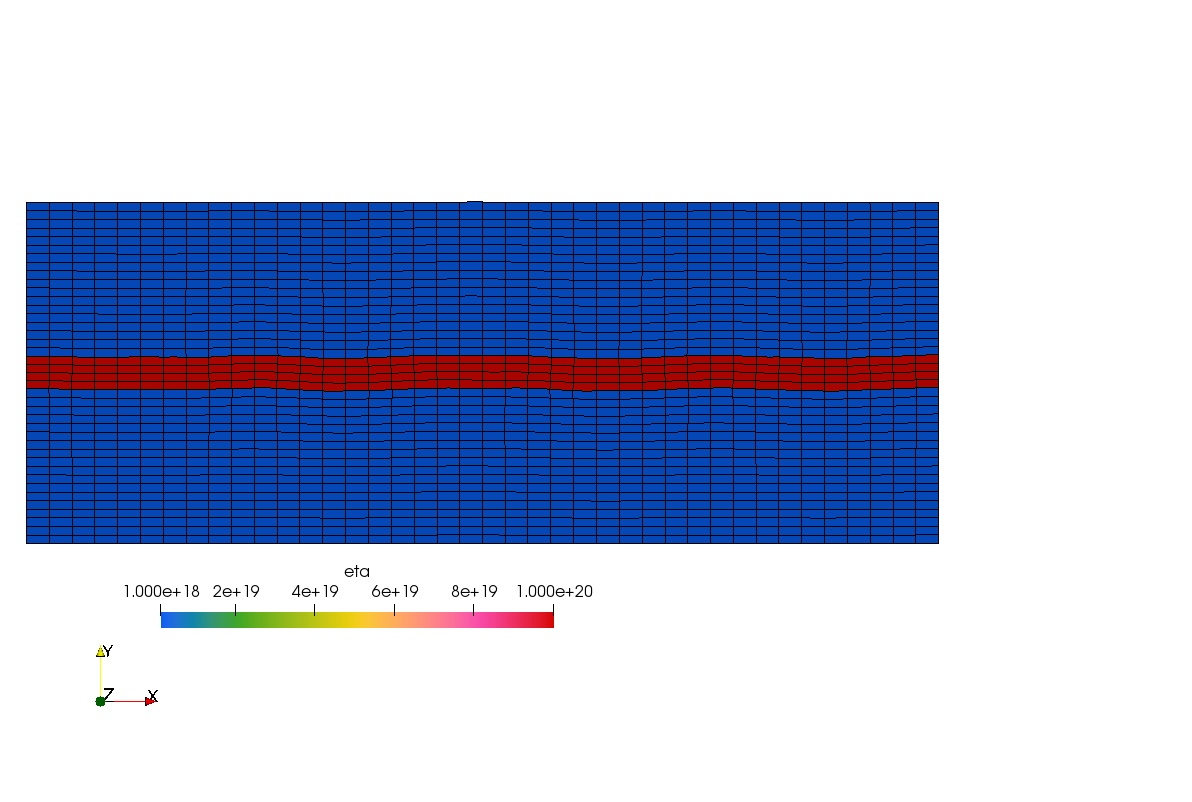
\includegraphics[width=3.4cm]{python_codes/fieldstone_129/results/experiment1/eta0199}
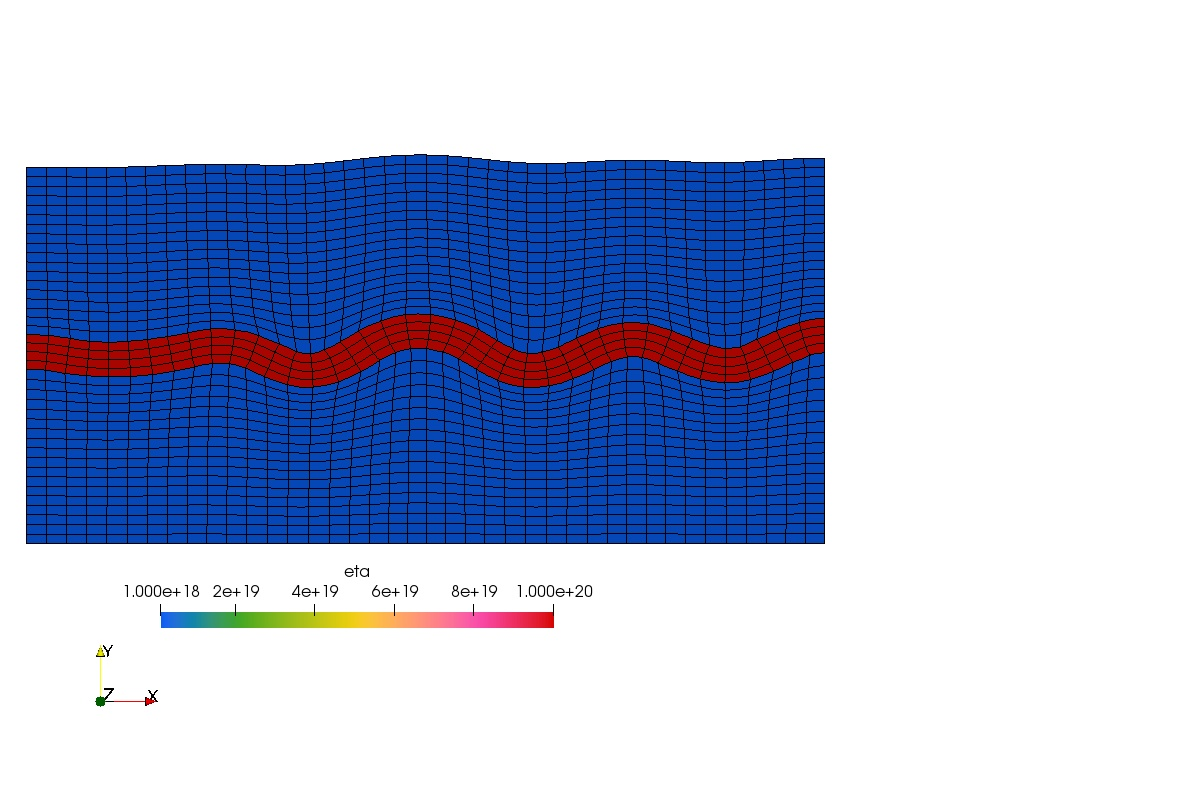
\includegraphics[width=3.4cm]{python_codes/fieldstone_129/results/experiment1/eta0299}
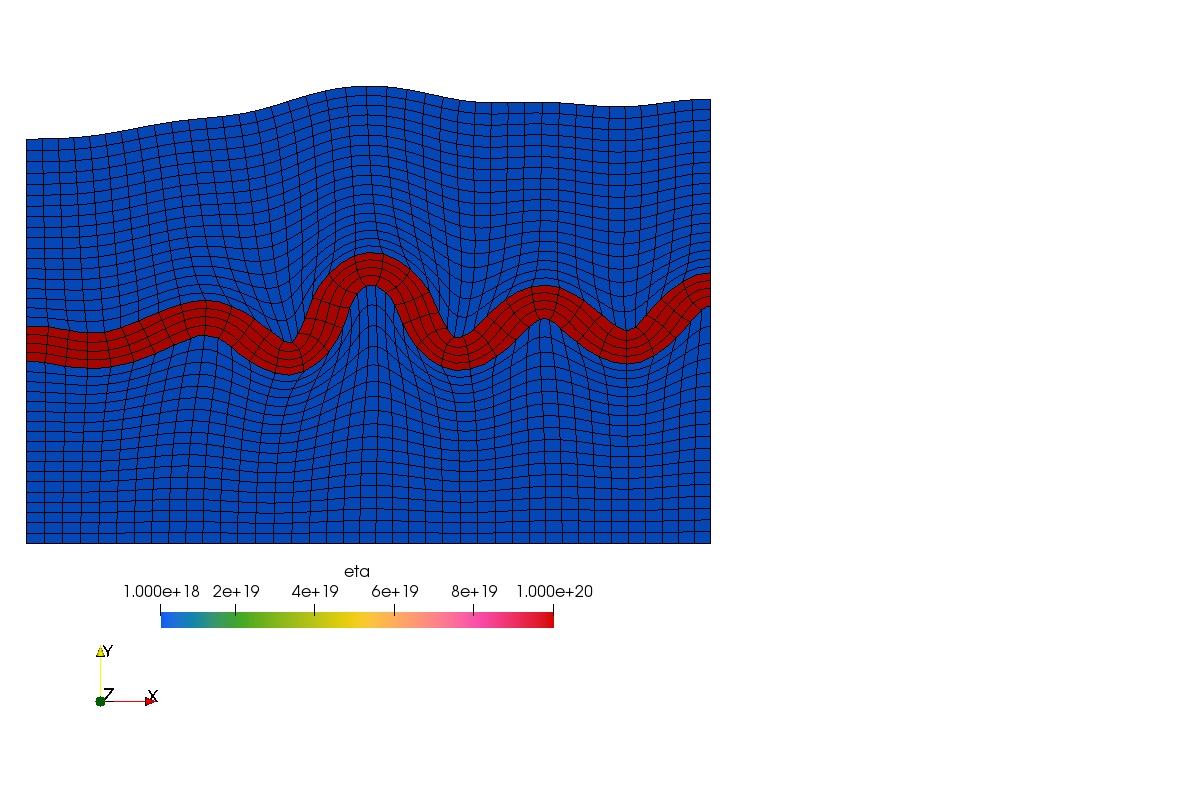
\includegraphics[width=3.4cm]{python_codes/fieldstone_129/results/experiment1/eta0399}\\
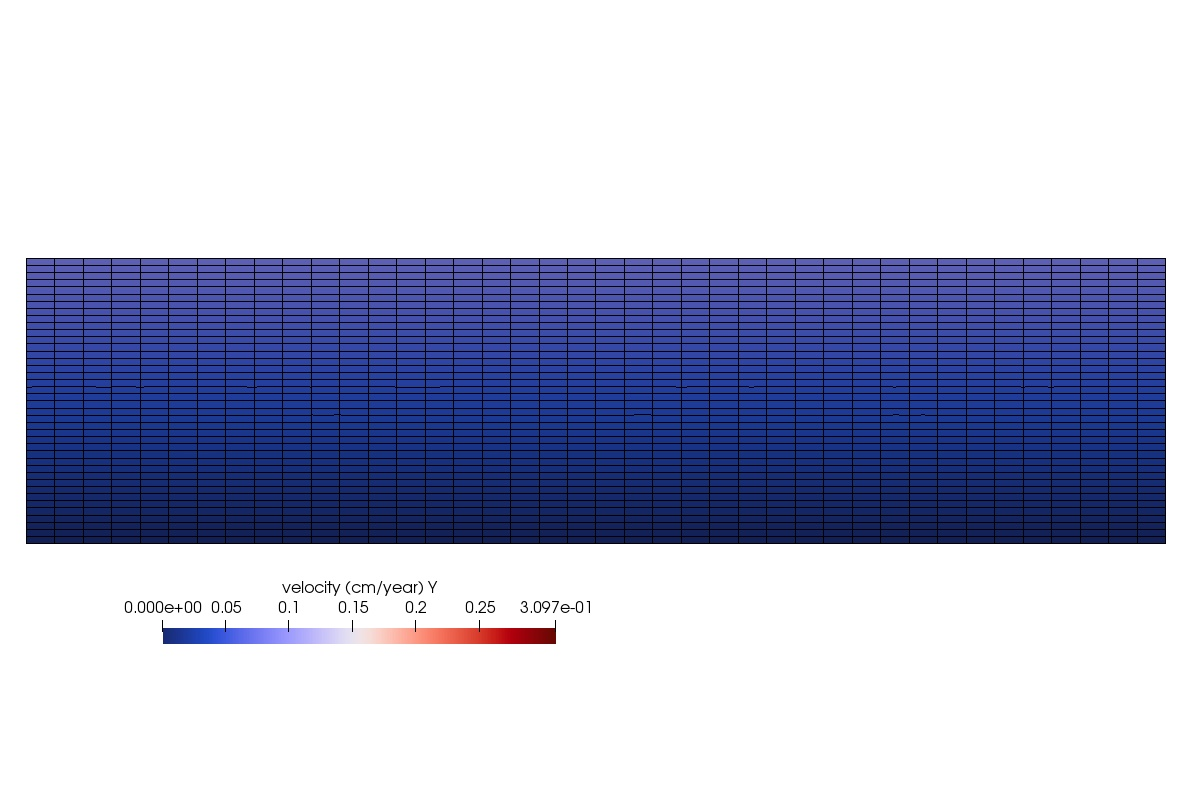
\includegraphics[width=3.4cm]{python_codes/fieldstone_129/results/experiment1/vel0000}
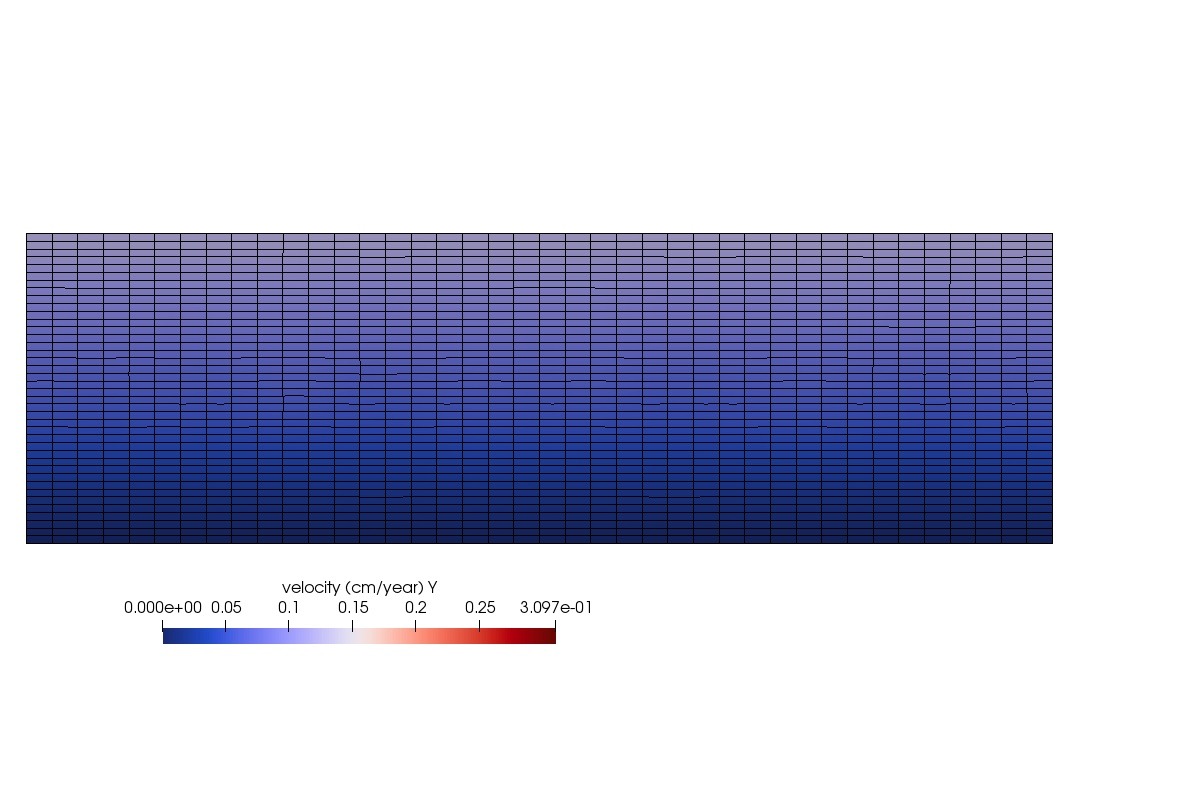
\includegraphics[width=3.4cm]{python_codes/fieldstone_129/results/experiment1/vel0099}
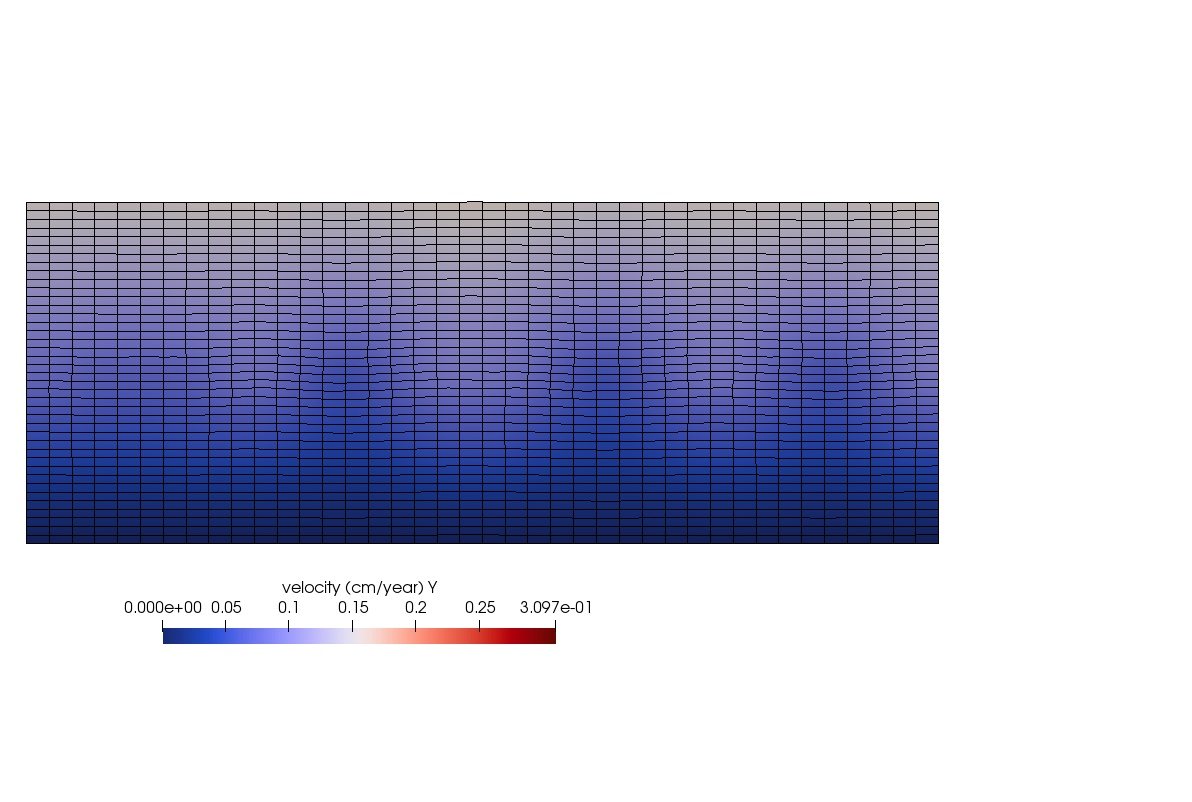
\includegraphics[width=3.4cm]{python_codes/fieldstone_129/results/experiment1/vel0199}
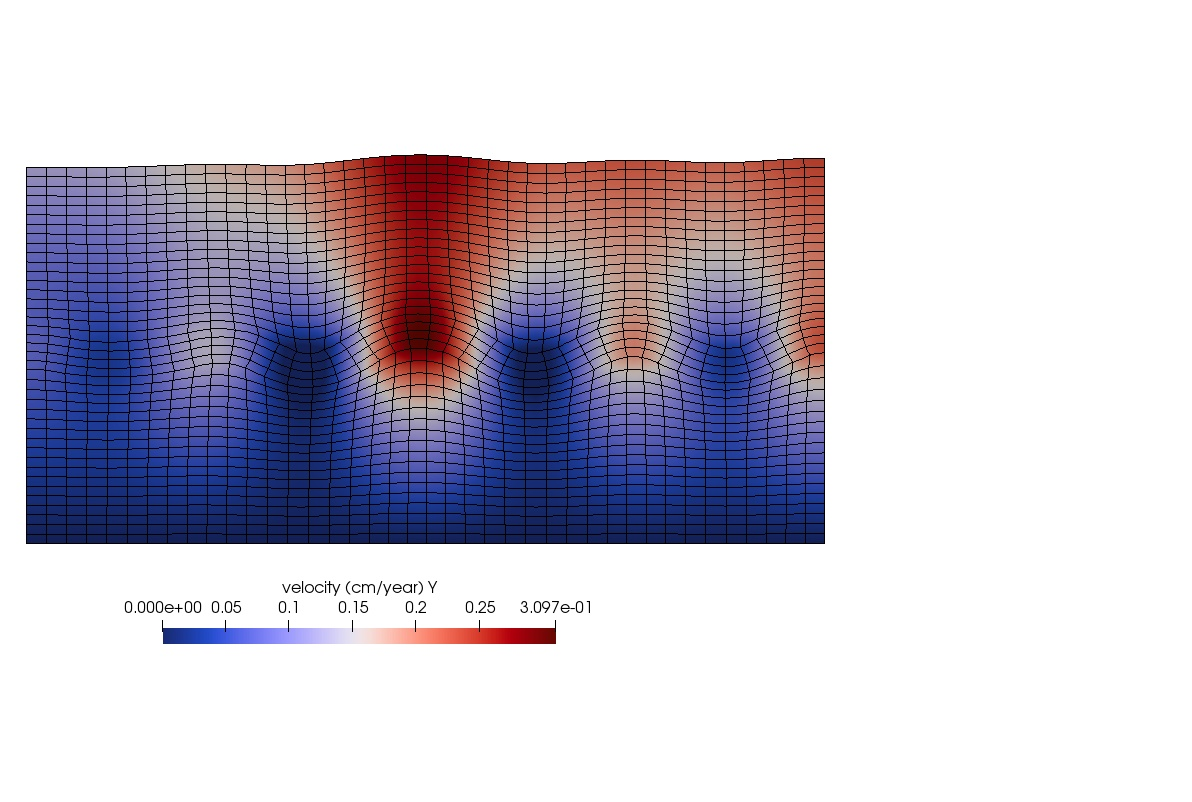
\includegraphics[width=3.4cm]{python_codes/fieldstone_129/results/experiment1/vel0299}
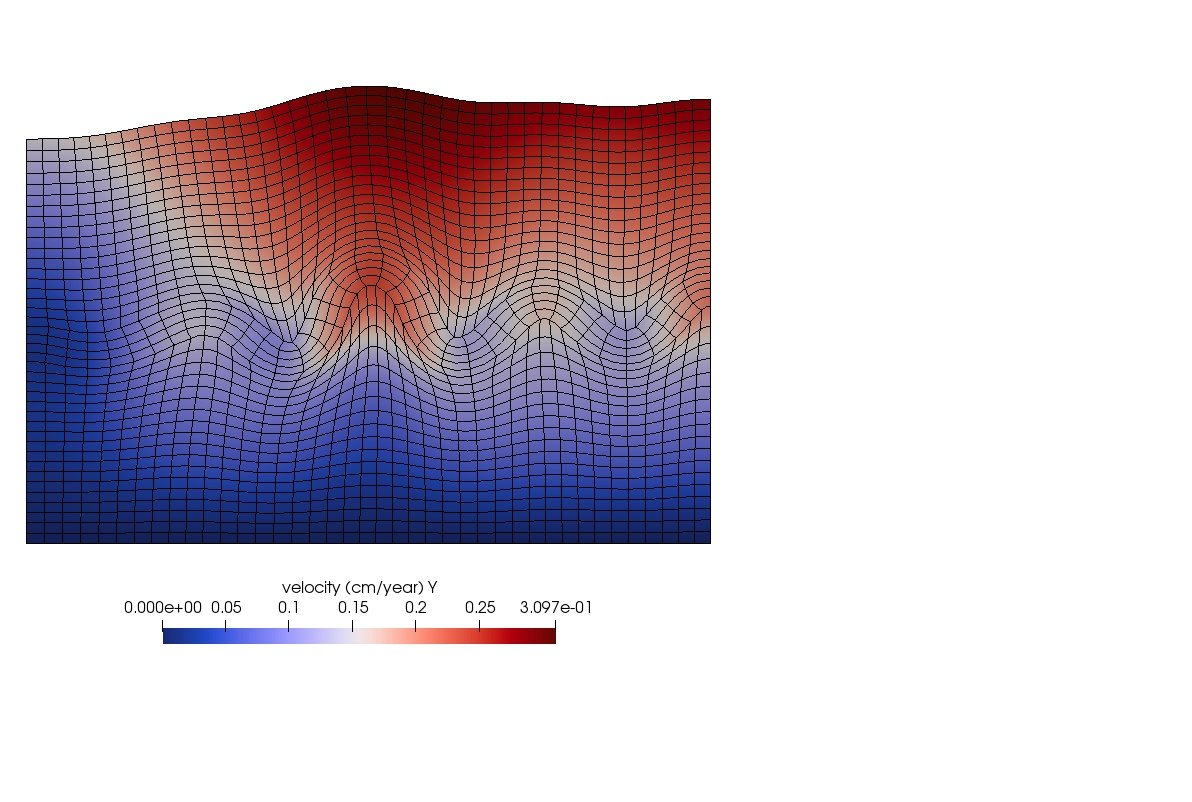
\includegraphics[width=3.4cm]{python_codes/fieldstone_129/results/experiment1/vel0399}\\
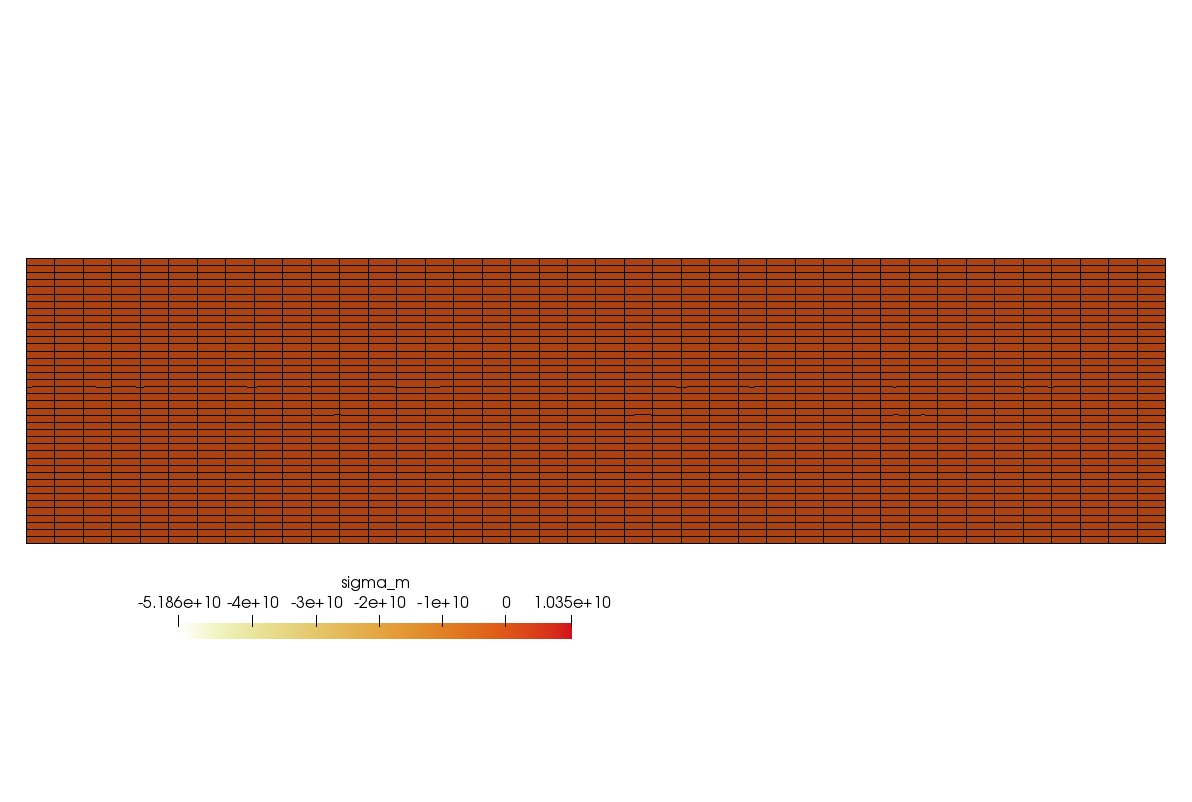
\includegraphics[width=3.4cm]{python_codes/fieldstone_129/results/experiment1/sigmam0000}
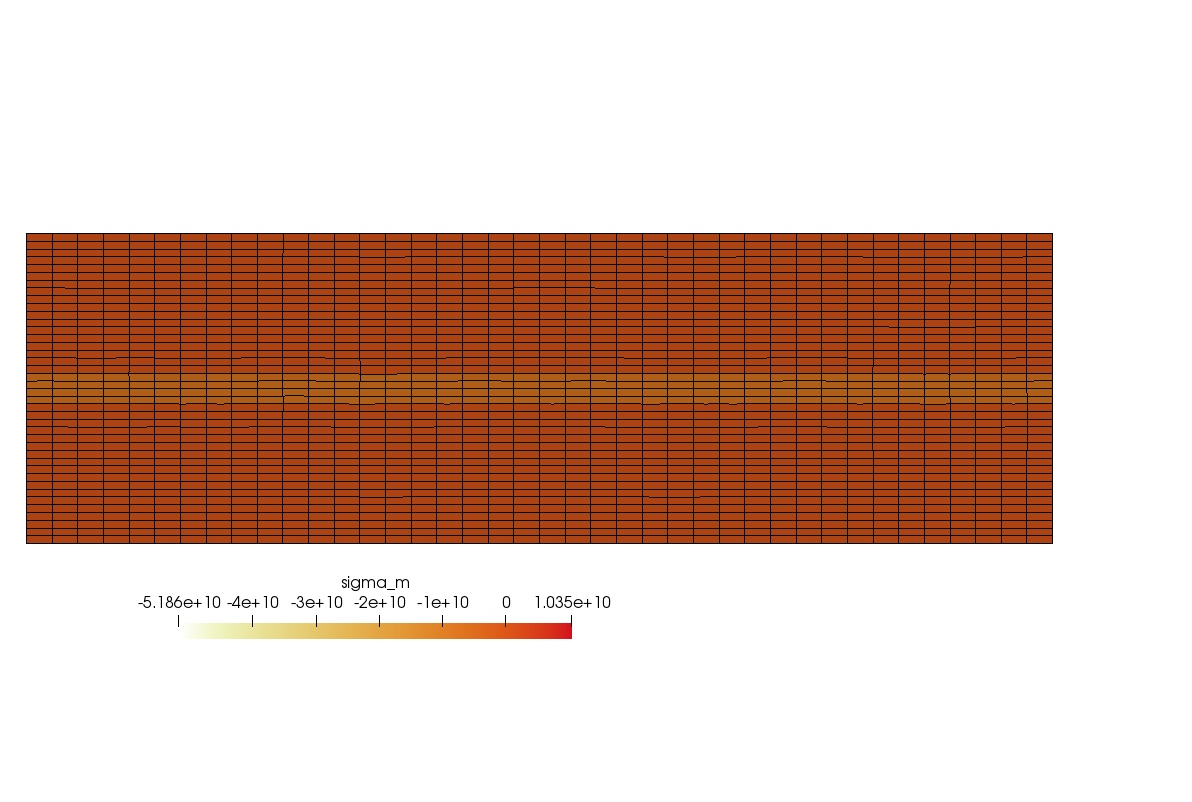
\includegraphics[width=3.4cm]{python_codes/fieldstone_129/results/experiment1/sigmam0099}
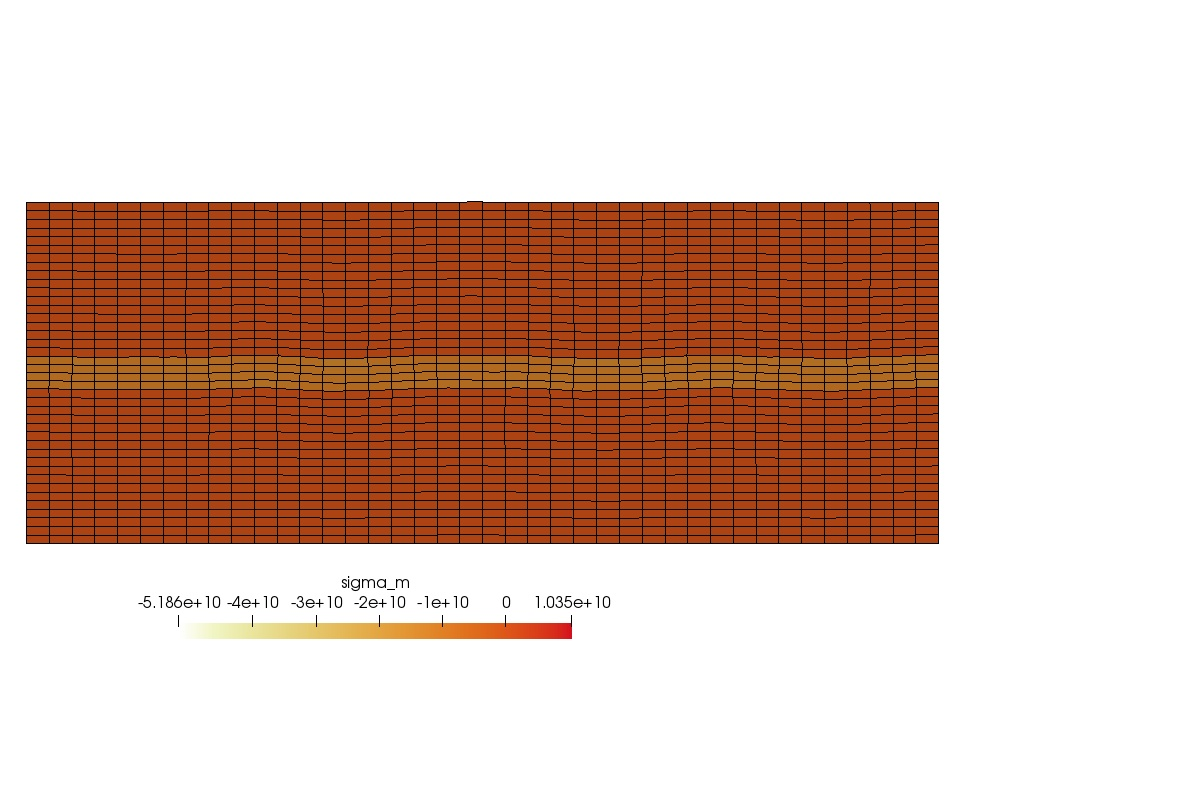
\includegraphics[width=3.4cm]{python_codes/fieldstone_129/results/experiment1/sigmam0199}
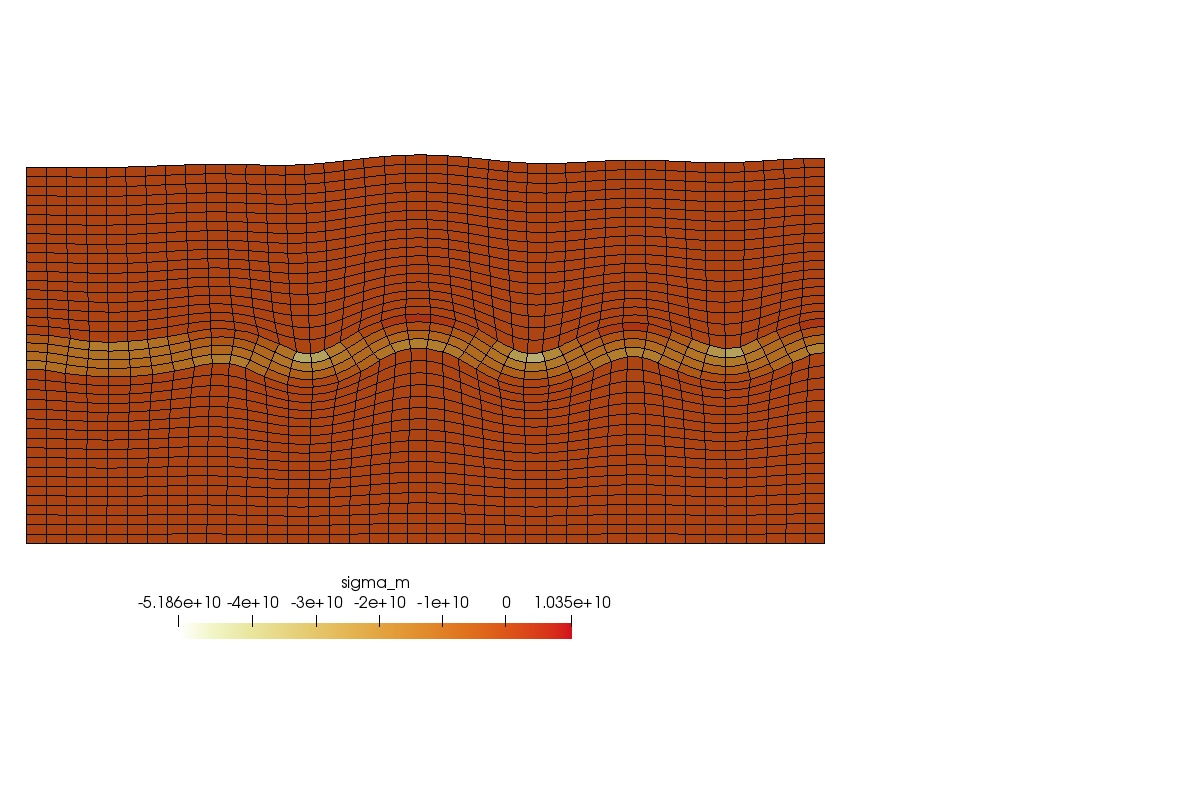
\includegraphics[width=3.4cm]{python_codes/fieldstone_129/results/experiment1/sigmam0299}
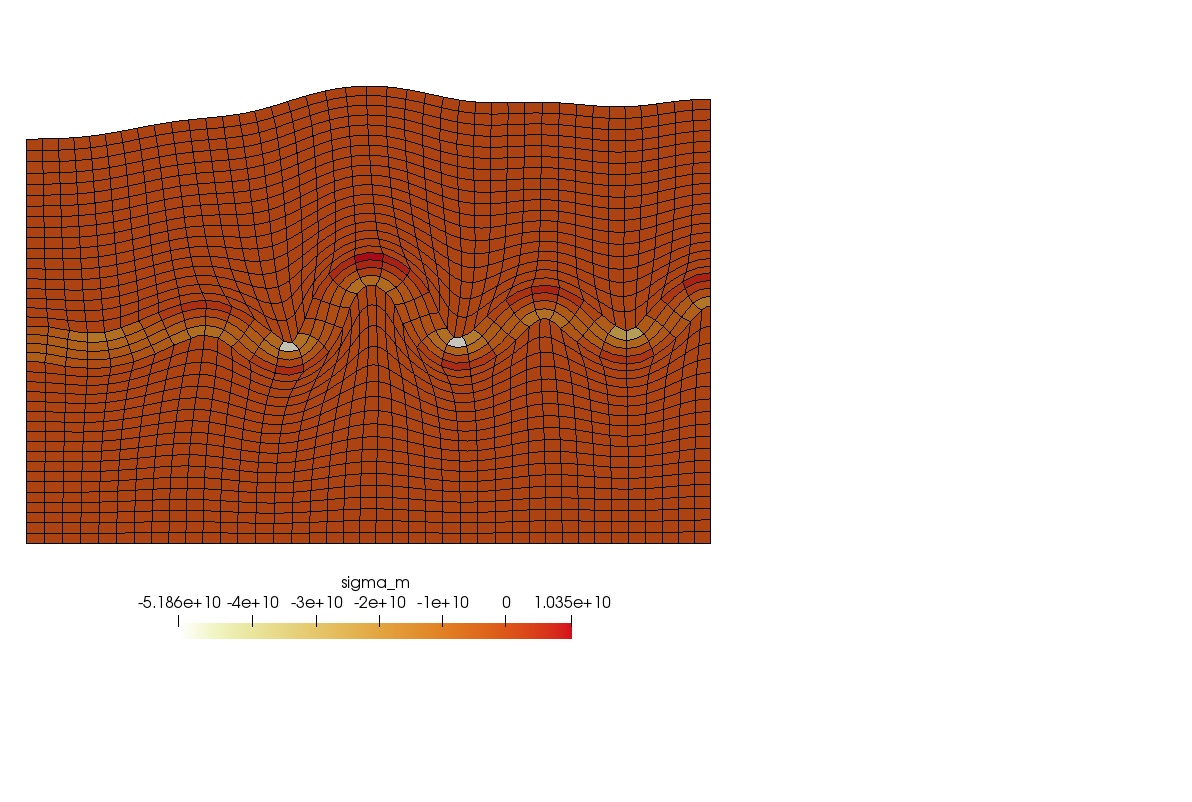
\includegraphics[width=3.4cm]{python_codes/fieldstone_129/results/experiment1/sigmam0399}\\
\end{center}

{\color{red} this experiment works fine, elastic properties constant in space,
only viscous props vary}

\newpage
%------------------------------------------------------------------------------
\subsection*{Analytical benchmark - pure shear (experiment=2)}

The domain is $\SI{50}{\km}\times\SI{50}{\km}$. There is a single 
material in the domain characterised by $\eta=\SI{1e21}{\pascal\second}$,
$\mu=\SI{1e10}{\pascal}$. The time step is $\delta t=100~\si{\year}$.
Boundary conditions are free slip on all sides, with $u=+\SI{1}{\cm\per\year}$
on the right and $v=-\SI{1}{\cm\per\year}$ on the top.

The unstressed, {\it incompressible} viscoelastic Maxwell medium is subjected to a velocity field 
resulting in pure shear. 
The increase of the accumulated stress with time is given by an analytical solution:
\begin{equation}
{\bm \tau} 
= 2\eta\ {\dot{\bm \varepsilon}} \left ( 1-\exp\left(-\frac{\mu }{\eta} t \right) \right )
= 2\eta\ {\dot{\bm \varepsilon}} \left ( 1-\exp\left(-\frac{t}{t_M} \right) \right )
\end{equation}
where the Maxwell time is $t_M = \frac{\eta}{\mu} = \SI{1e11}{\second} \simeq 3171~\si{\year}$.

\begin{center}
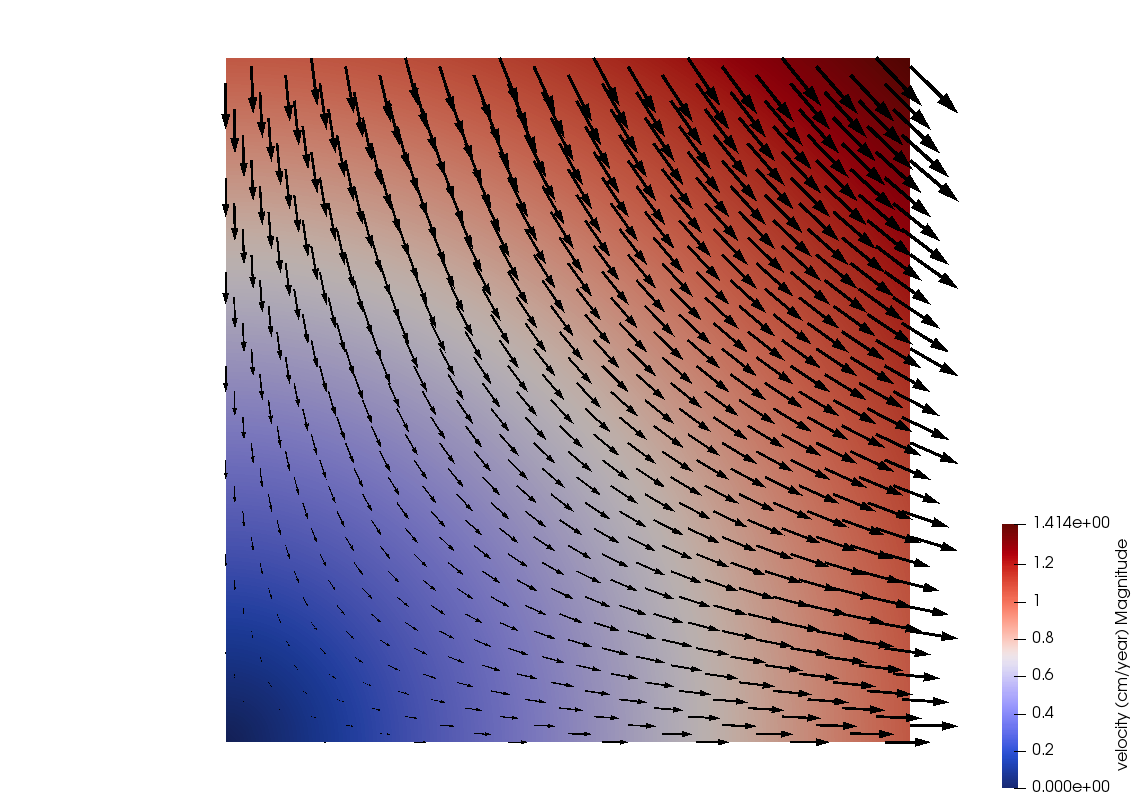
\includegraphics[width=5.7cm]{python_codes/fieldstone_129/results/experiment2/vel}\\
{\captionfont Velocity field.}
\end{center}

We have 
\[
\eta_{eff} 
= \frac{\eta \delta t}{\delta t + \eta/\mu} 
= \frac{10^{21} \cdot 3.154\times 10^{9}}{3.154\times 10^{9} + 10^{21}/10^{10}} 
\simeq 
\SI{3.0592e19}{\pascal\second} 
\]

The resolution is set to $10\times 10$ elements. 200 time steps are carried out.

\begin{center}
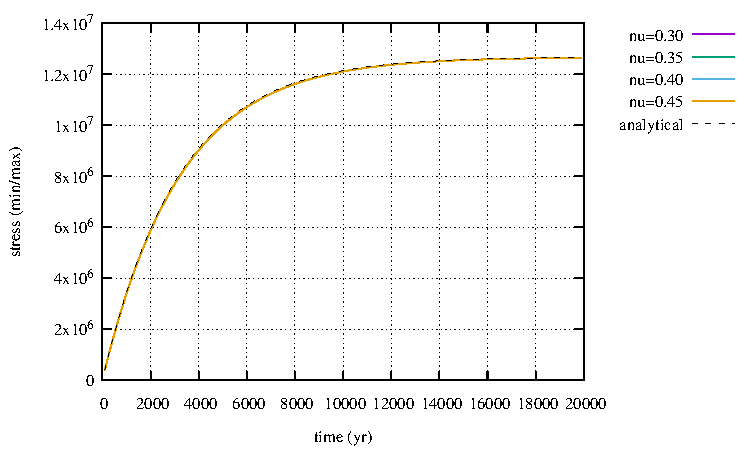
\includegraphics[width=8cm]{python_codes/fieldstone_129/results/experiment2/stats_stress}\\
{\captionfont Evolution or $\sigma_{xx}$ statistics over 20~kyr for various values of $\nu$.}
\end{center} 

\newpage
%------------------------------------------------------------------------------
\subsection*{Analytical benchmark (experiment=6)}

This is an extremely simple setup. The domain contains a single material. 
Boundary conditions are free slip on left, right and bottom, stress-free boundary conditions 
at the top. 

The domain is 50x50km, gravity is $\vec{g}=-9.81~\si{\meter\per\square\second}$, 
$\eta=10^{21}$, $\rho=3300$, $\mu=10^{10}$.

We expect the system to compact under its own weight and reach a 
steady state. FIND OUT !!





\newpage
%------------------------------------------------------------------------------
\subsection*{Numerical benchmark - Bending of elastic slab (experiment=3)}

This benchmark is a numerical benchmark, but not an analytical one. 
It originates in Taras Gerya's book. It is originally for incompressible visco-elastic fluids so we will run it at different values of the Poisson ratio parameter.
It is also carried out in \stone~64.

The sinking slab benchmark consists of a beam of elastic material which is placed 
in a weak and viscous surrounding medium. The initially unstressed beam is attached 
to the left domain boundary through boundary conditions. A stress is then applied to  
the beam in the form of gravity. The applied gravity force results in the deformation 
of the beam through bending. After 20 kyr, the gravity field is turned off and the 
elastic properties of the beam will then force itself to its original position.  
The set-up of the benchmark is given in the following figure: 

\begin{center}
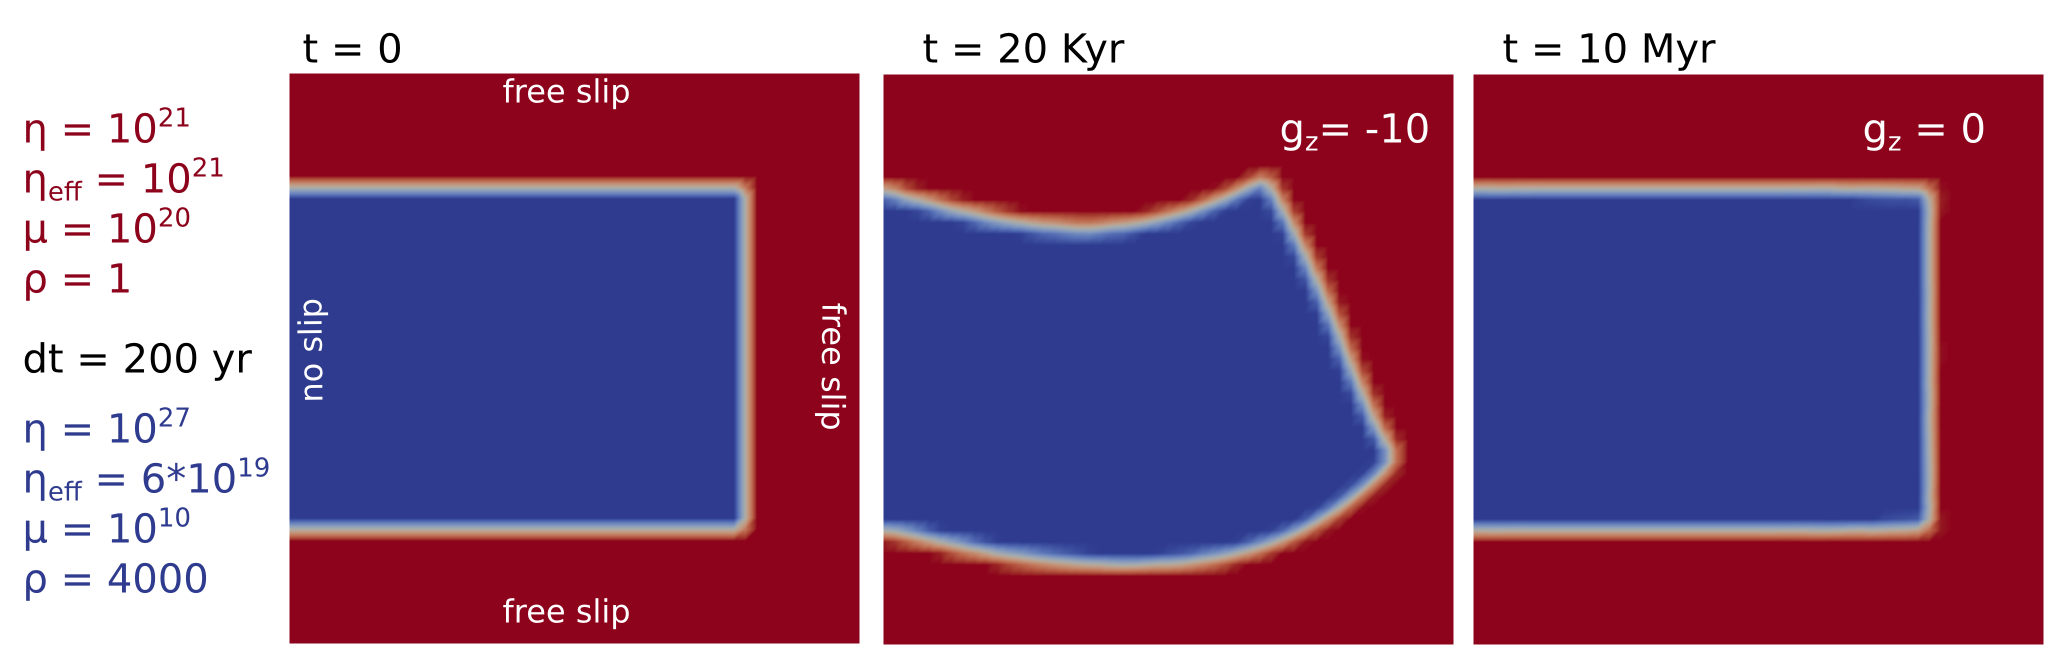
\includegraphics[width=6cm]{python_codes/fieldstone_64/images/poster_benchmark.png}\\
\captionfont{Set-up of the benchmark from \cite{gery10}. The properties of the 
two materials are given on the left, together\\ with the initial configuration of the benchmark.} 
\end{center}

The 800x600km beam is surrounded by a low-density, low-viscosity and high shear modulus medium 
of which the specifications are given in  the following table.
The boundary conditions of the domain consist of a no slip condition at  
the left boundary where the slab is attached and free slip boundary conditions along all other sides. 
The results are calculated on a grid with a resolution of 50x50 elements.
The time step is set to $\delta t = 200yr$ (i.e. gravity is switched off after 100 time steps).

As explained in the book: ``
The slab deformation is purely elastic due to the large Maxwell time (3 170 000 kyr) of slab material
compared to the total deformation time (20 000 kyr). In contrast, the low viscosity medium
is subjected to irreversible, purely viscous deformation since its Maxwell time (\num{3.17e-10} kyr) 
is negligible compared to the deformation time.''

\begin{center}
\begin{tabular}{lll}
\hline 
\textit{Material properties}& \textit{Elastic slab (fluid 1)}  & \textit{Surrounding medium (fluid 2)} \\
\hline 
\hline
Density         $\rho$ \  [kg/m$^{3}$]            & 4000                    & 1     \\
Viscosity       $\eta$ \  [\si{\pascal\second}]    & $10^{27}$               &   $10^{21}$     \\
Shear modulus   $\mu $ \  [\si{\pascal}]           & $10^{10}$               & $10^{20}$       \\
Maxwell time $t_M$     \  [yr]                     & 3.17Gyr                 &  $3.17\times10^{-7}$yr       \\
eff. visc.      $\eta_{eff}$ \ [\si{\pascal\second}] & 6.307199602192306e+19   &  9.999999984145105e+20      \\
\hline
\end{tabular}
\end{center}


\begin{center}
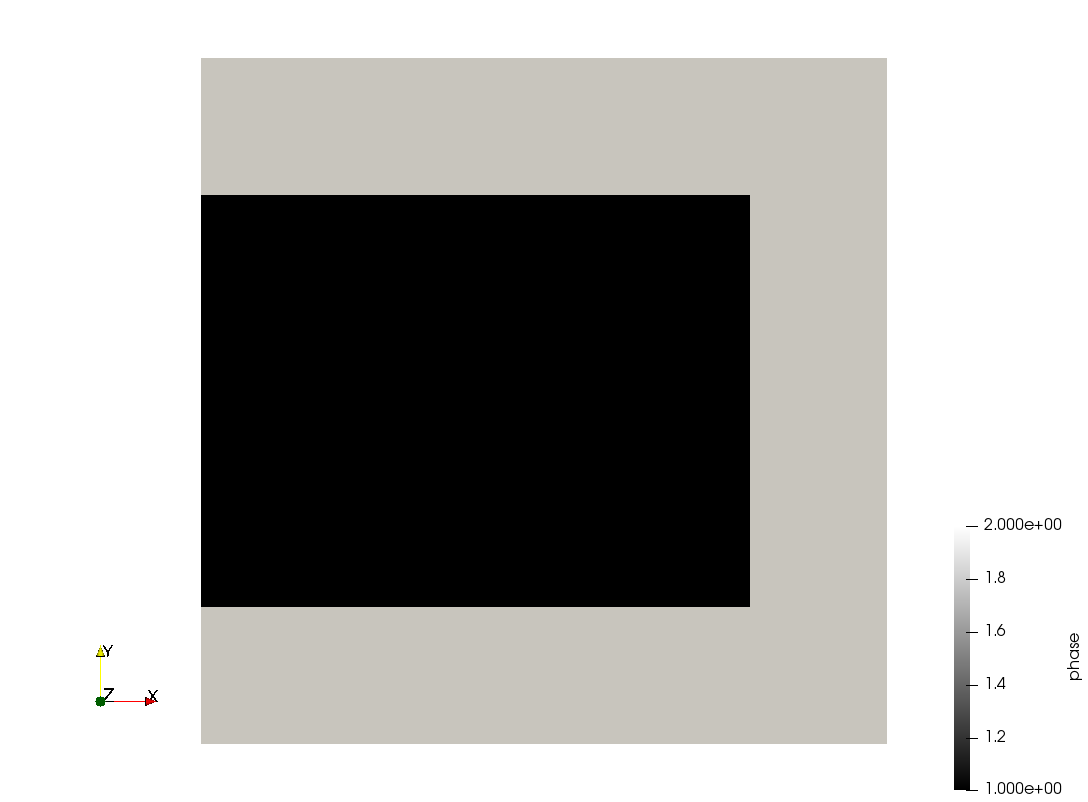
\includegraphics[width=5.7cm]{python_codes/fieldstone_129/results/experiment3/phase}
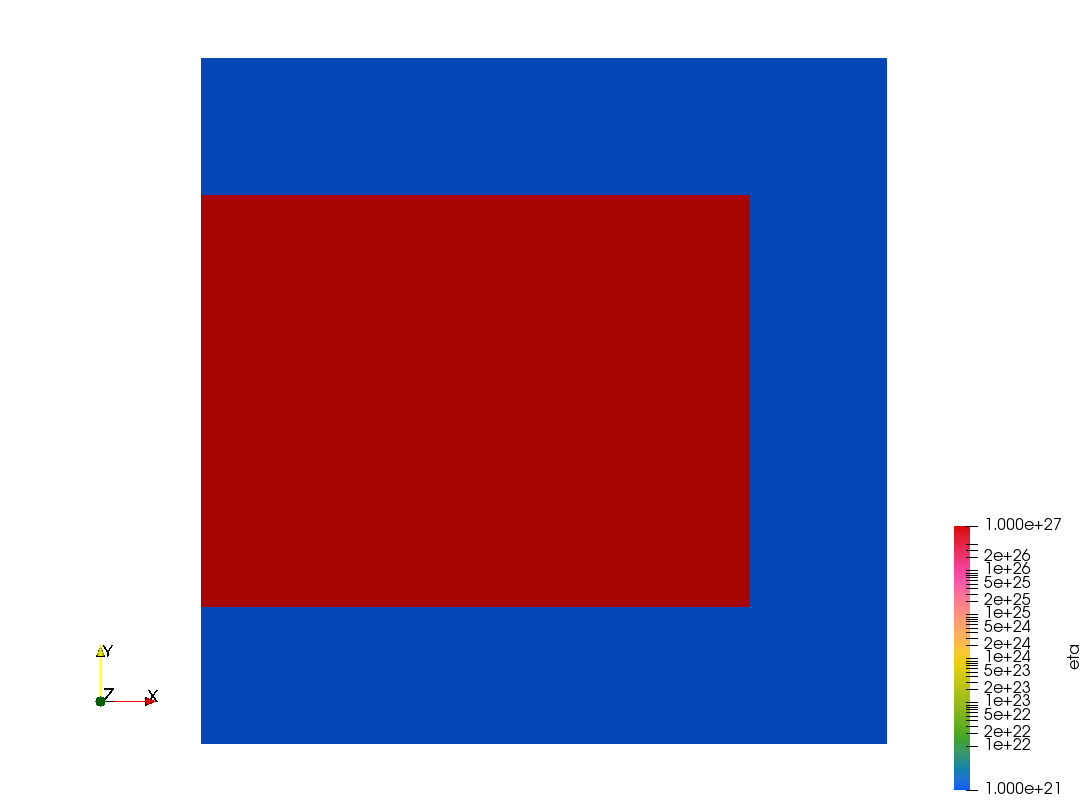
\includegraphics[width=5.7cm]{python_codes/fieldstone_129/results/experiment3/eta}
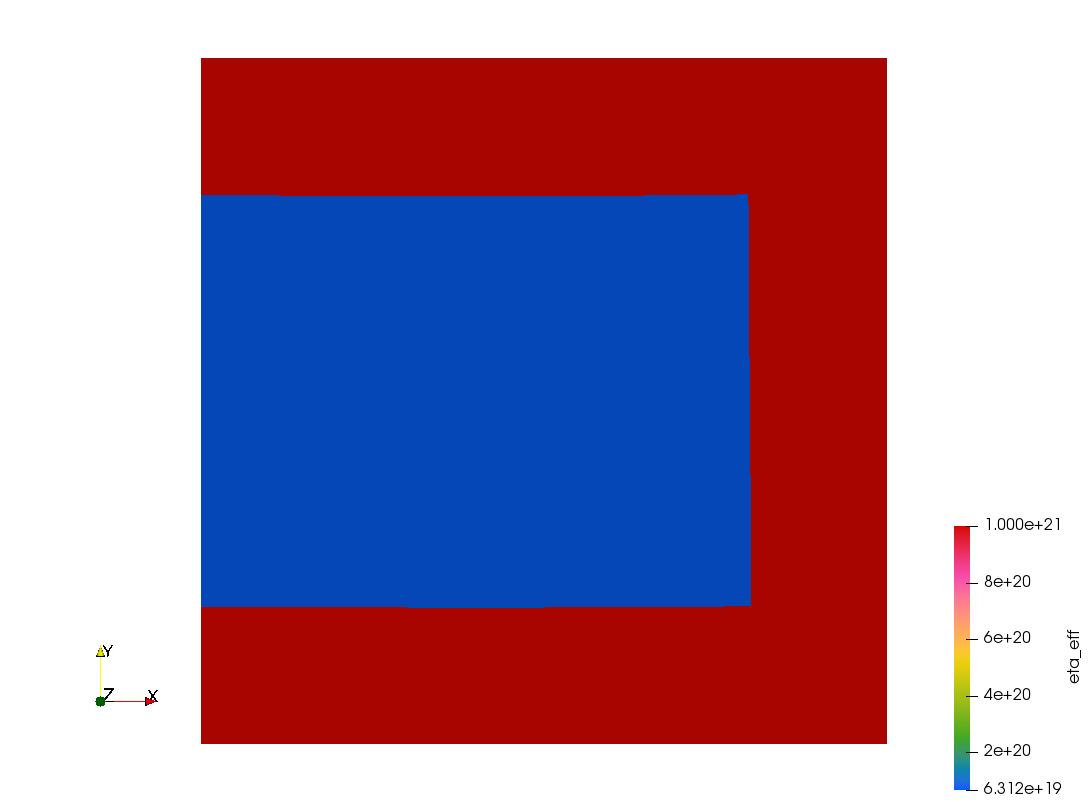
\includegraphics[width=5.7cm]{python_codes/fieldstone_129/results/experiment3/etaeff}\\
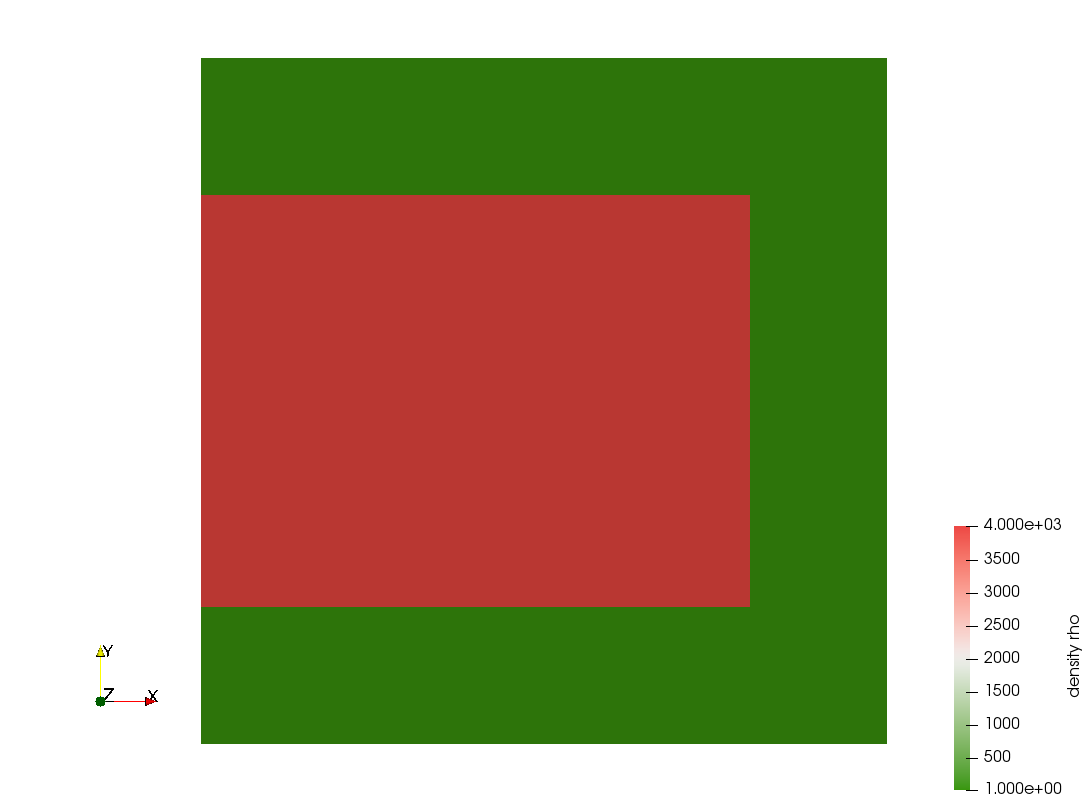
\includegraphics[width=5.7cm]{python_codes/fieldstone_129/results/experiment3/rho}
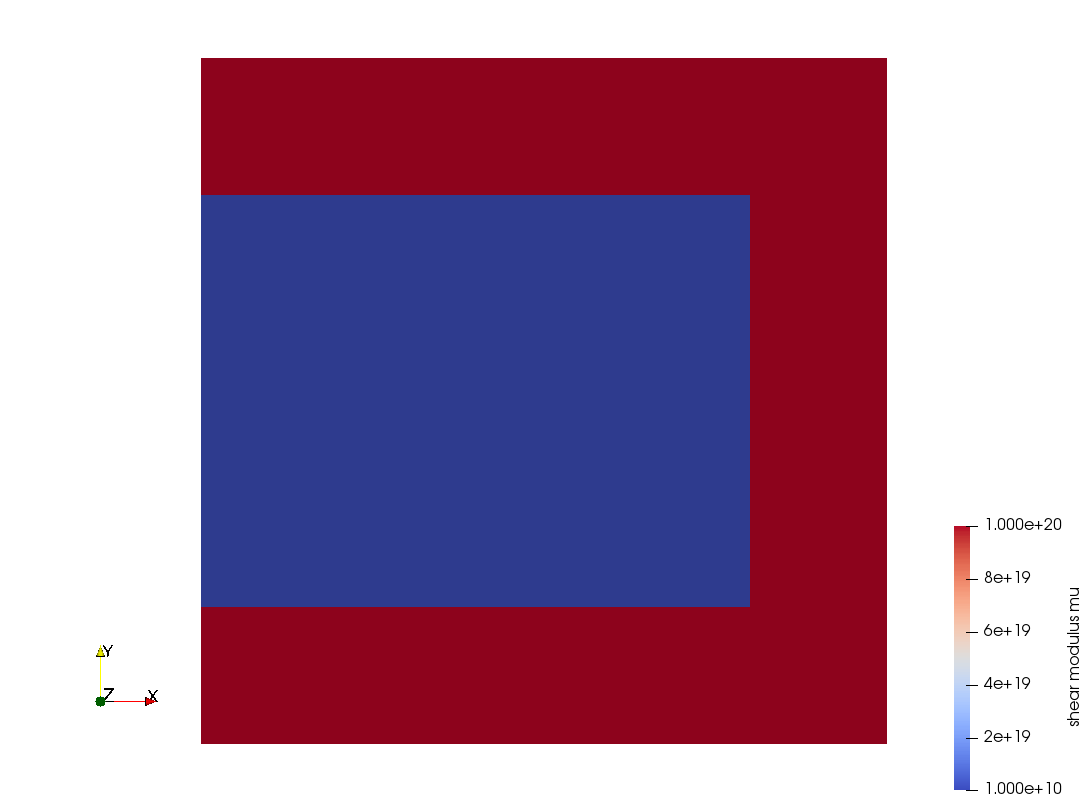
\includegraphics[width=5.7cm]{python_codes/fieldstone_129/results/experiment3/mu}
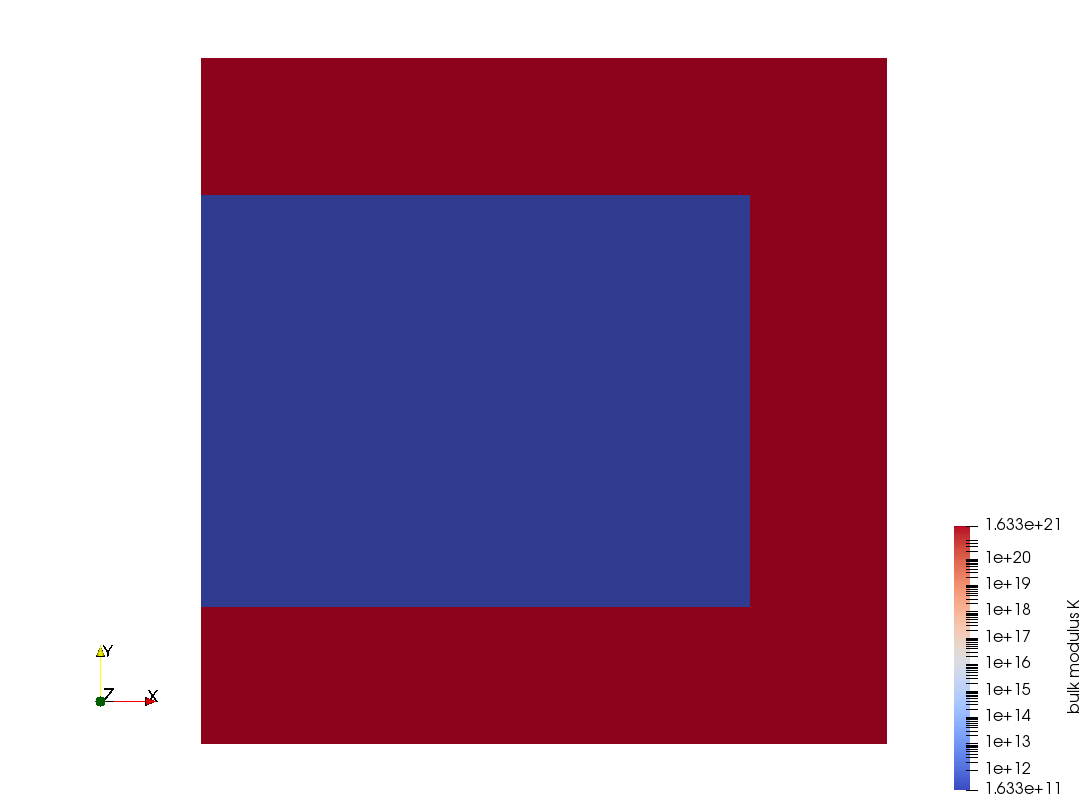
\includegraphics[width=5.7cm]{python_codes/fieldstone_129/results/experiment3/K}\\
{\captionfont Initial setup of the experiment.}
\end{center} 

Unfortunately this simulation explodes no matter the poisson ratio value.
It kinda looks like things go mostly wrong in the purely viscous part?

Here is a tentative analysis of what is going on. Let us look at the 
$\tilde{\bm D}$ for both phases (phase 1 is the slab -purely elastic, phase 2 is the fluid -purely viscous):
\[
\tilde{\bm D}_{phase=1} = 
\left(
\begin{array}{ccc}
2.003e+20 &7.409e+19 & 0 \\
7.409e+19  & 2.003e+20 & 0 \\
0 & 0 & 6.311e+19 
\end{array}
\right)
\qquad
\tilde{\bm D}_{phase=2} = 
\left(
\begin{array}{ccc}
1.161e+30 & 1.161e+30 & 0 \\
1.161e+30 & 1.161e+30 & 0 \\
0 & 0 & 9.999e+20
\end{array}
\right)
\]

\[
{\bm D}_{s,phase=1} = 
\left(
\begin{array}{ccc}
0.999    & 2.103e-08 & 0 \\
2.103e-08 & 0.999    & 0 \\
0 & 0 & 0.999
\end{array}
\right)
\qquad
{\bm D}_{s,phase=2} = 
\left(
\begin{array}{ccc}
0.333 & 0.333 & 0 \\ 
0.333 & 0.333 & 0 \\
0 & 0 & 1.584e-09
\end{array}
\right)
\]
In this case we see that we have more than 10 orders of magnitude of 
difference between the coefficients of the $\tilde{\bm D}_s$ matrices.
This is obviously bad news and is likely the cause of the problems
experienced. 

In order to insure that the fluid is behaving viscously, all we need to have 
is $\mu \delta t >> \eta$. In this case, we have 
$\mu \delta t = 10^{20} \cdot 200 \cdot 3600 \cdot 365 \cdot 24 \simeq 6.3\times 10^{29}$
while $\eta=10^{21}$ and we have seen that the Maxwell time is then $3.17\times10^{-7}~\si{\year}$.

However one could argue that $\mu \delta t / \eta \simeq 6.3\times 10^{8}$ is overkill. 
Let us then impose $\mu \delta t / \eta \simeq 6.3\times 10^{3}$, i.e. let us take $\mu=10^{15}$.

The stress fields look smoother, but there are still rather wild oscillations!!!

{\color{red} is there a bug or is this a feature of this formulation? } 
I NEED BENCHMARKS!!!

Rob metioned a paper by Melosh?



\newpage
%------------------------------------------------------------------------------
\subsection*{Numerical benchmark - Flexure of elastic plate (experiment=4)}

This benchmark is presented in \textcite{chtl13}. 

\begin{center}
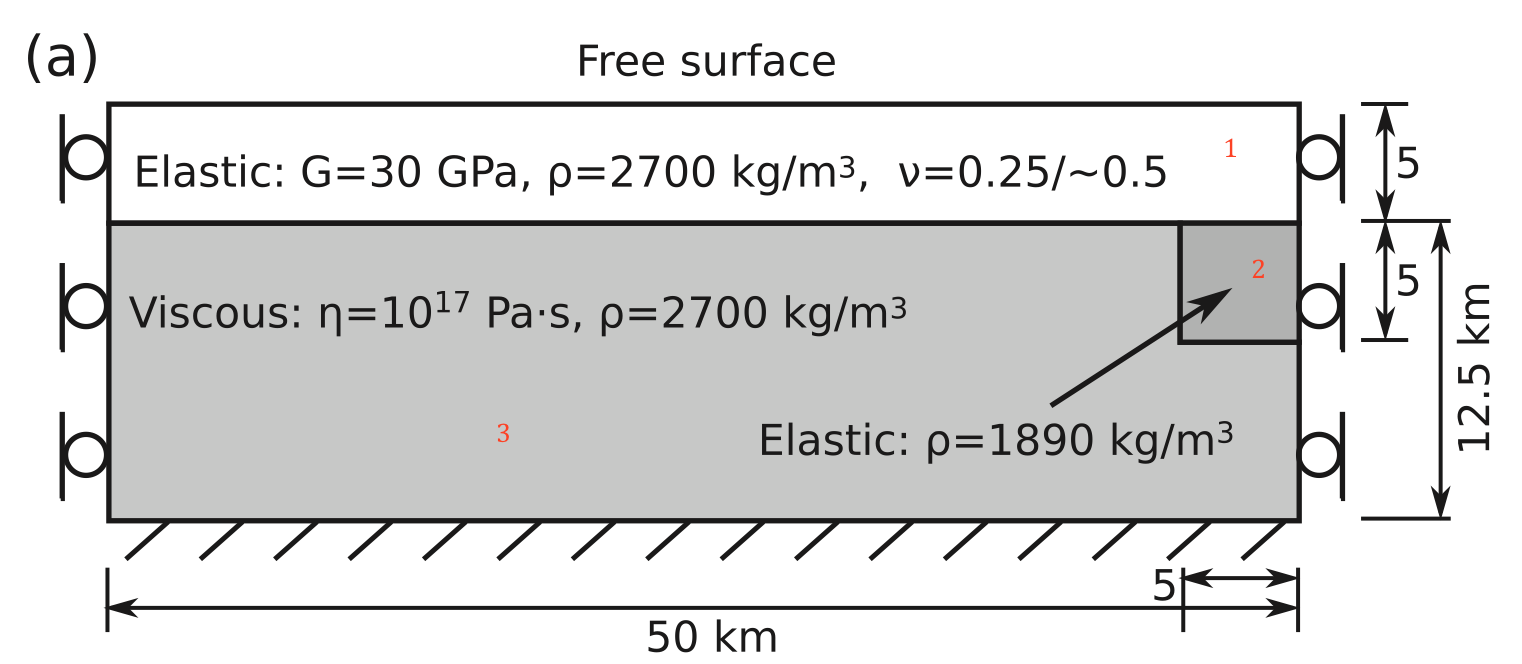
\includegraphics[width=9cm]{python_codes/fieldstone_129/images/chtl13a}
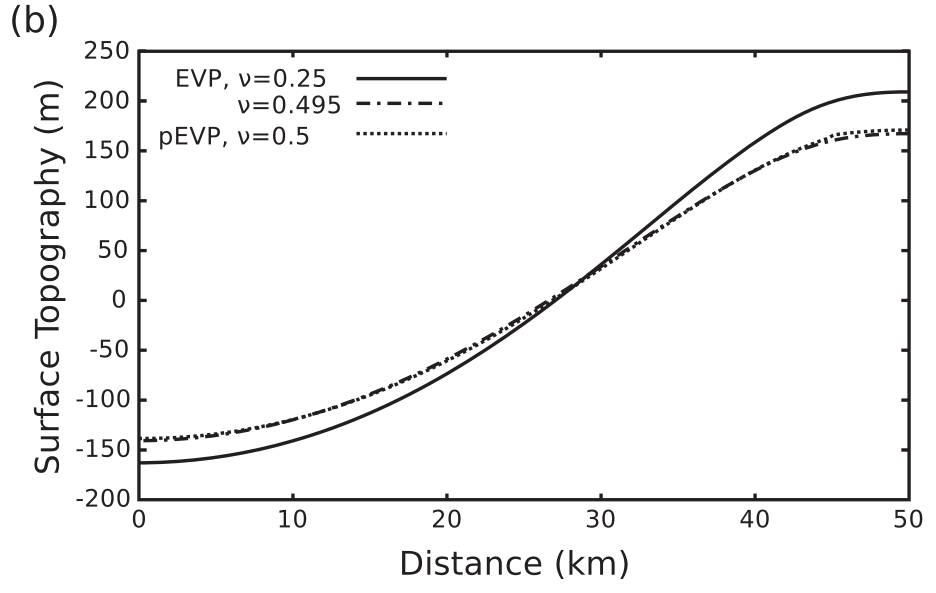
\includegraphics[width=7cm]{python_codes/fieldstone_129/images/chtl13b}\\
{\captionfont 
Taken from \textcite{chtl13}. ``Effect of elastic compressibility on the prediction 
of an elastic thin plate subject to an uplifting load. (a)
Model setup for a finite length elastic layer subjected to a
finite length buoyant load applied on the bottom. (b) Profiles
of mean-subtracted surface topography.''}
\end{center}


\begin{center}
\begin{tabular}{llll}
\hline 
\textit{Material properties}& \textit{elastic plate (1)}  & \textit{elastic block (2)} & \textit{viscous mantle (3)} \\
\hline 
\hline 
Density         $\rho$       \ \si{\kg\per\cubic\meter} & 2700&1890 &2700 \\  
Viscosity       $\eta$       \ \si{\pascal\second}      & $10^{35}$& $10^{35}$ & $10^{17}$ \\  
Shear modulus   $\mu $       \ \si{\pascal}             & $30\cdot10^9$& $30\cdot10^9$&  $10^{50}$ \\
Maxwell time    $t_M$        \ \si{\year}               & 10569930 &  10569930 & 3.1709791983764584e-41 \\  
eff. visc.      $\eta_{eff}$ \ \si{\pascal\second}      & 4.73039776e+18& 4.73039776e+18&  1e+17\\ 
\hline 
\end{tabular} 
\end{center}

\begin{center}
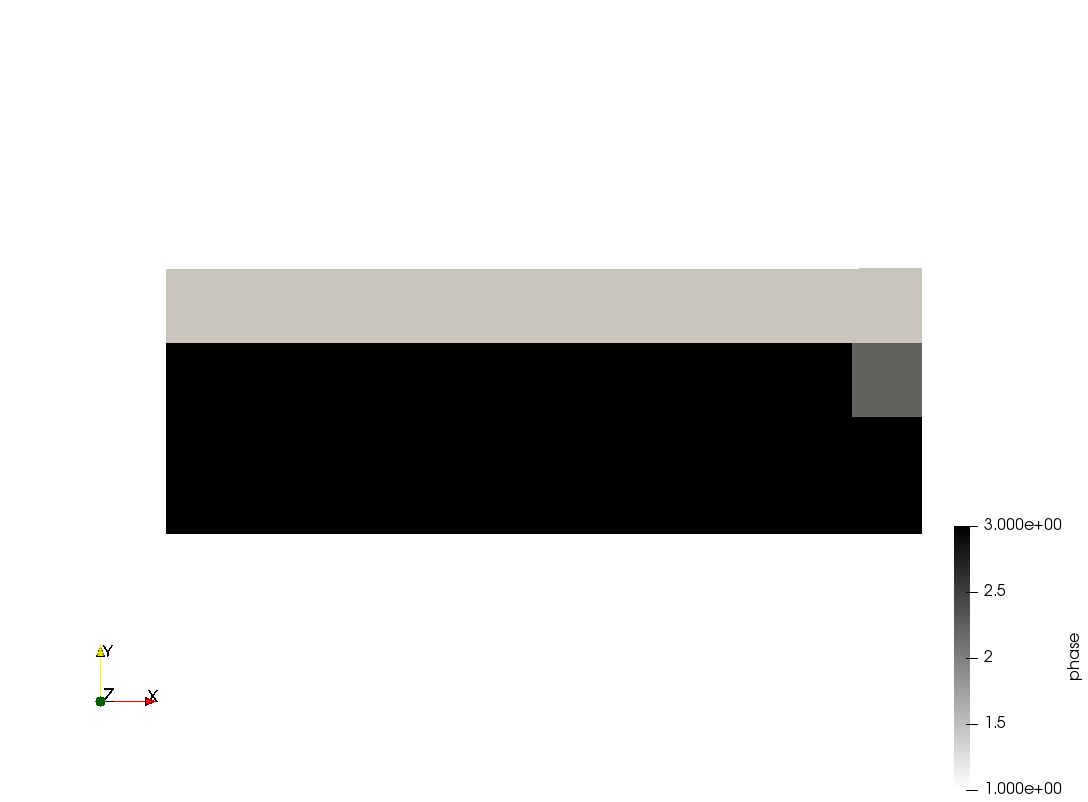
\includegraphics[width=5.7cm]{python_codes/fieldstone_129/results/experiment4/phase}
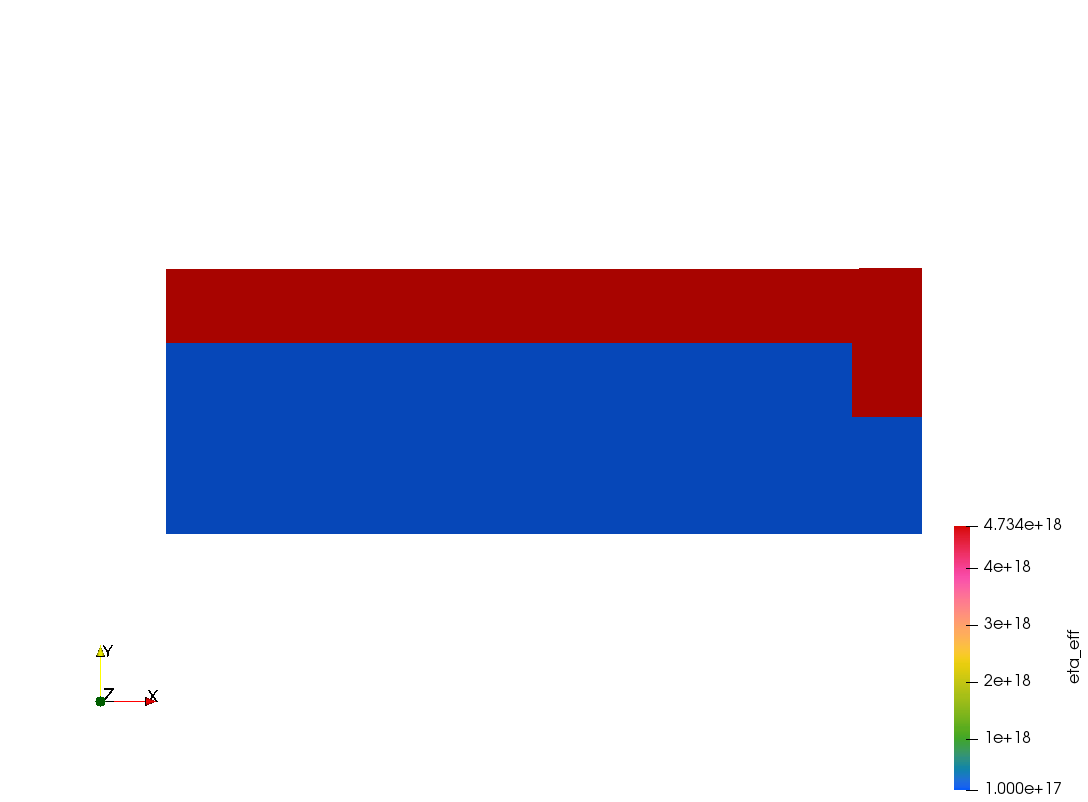
\includegraphics[width=5.7cm]{python_codes/fieldstone_129/results/experiment4/etaeff}
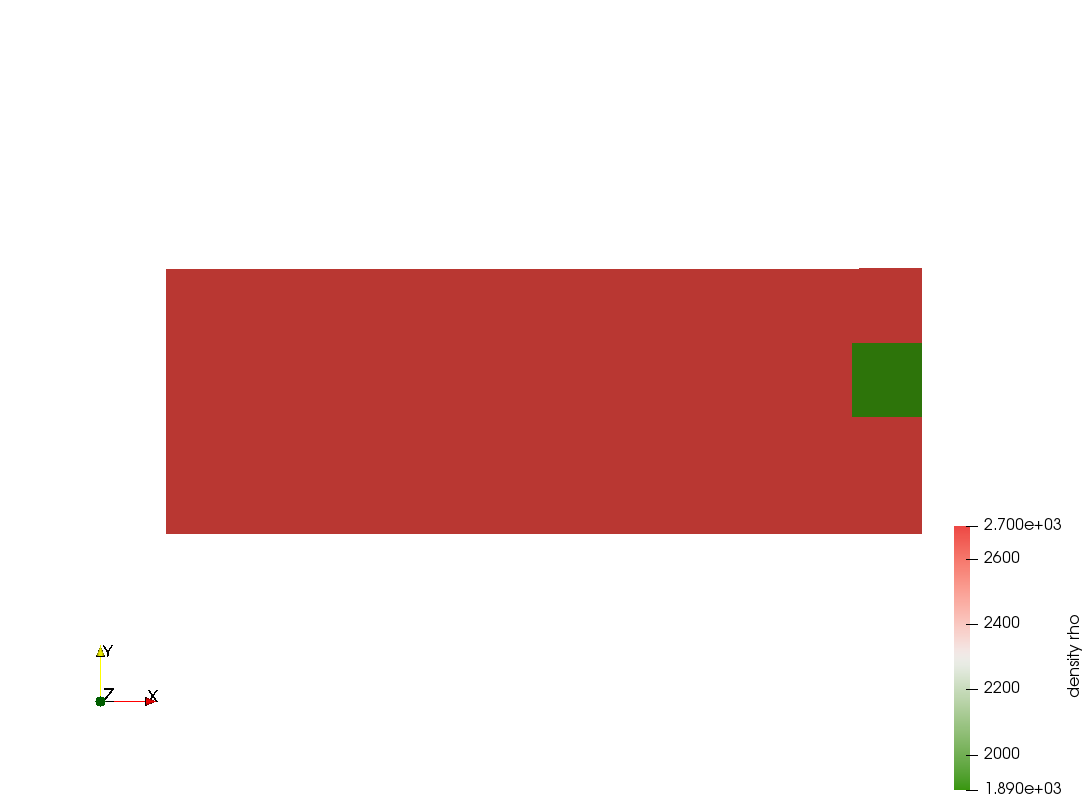
\includegraphics[width=5.7cm]{python_codes/fieldstone_129/results/experiment4/rho}\\
{\captionfont Initial setup of the experiment.}
\end{center} 


{\color{red}This explodes when shear modulus contrast becomes too big, i.e. when a material 
essentially becomes purely viscous by having its $\mu$ very large. }
It showcases oscillations at the beginning too!





\newpage
%------------------------------------------------------------------------------
\subsection*{Numerical benchmark - Parallel-plate viscosimeter (experiment=5)}

\begin{center}
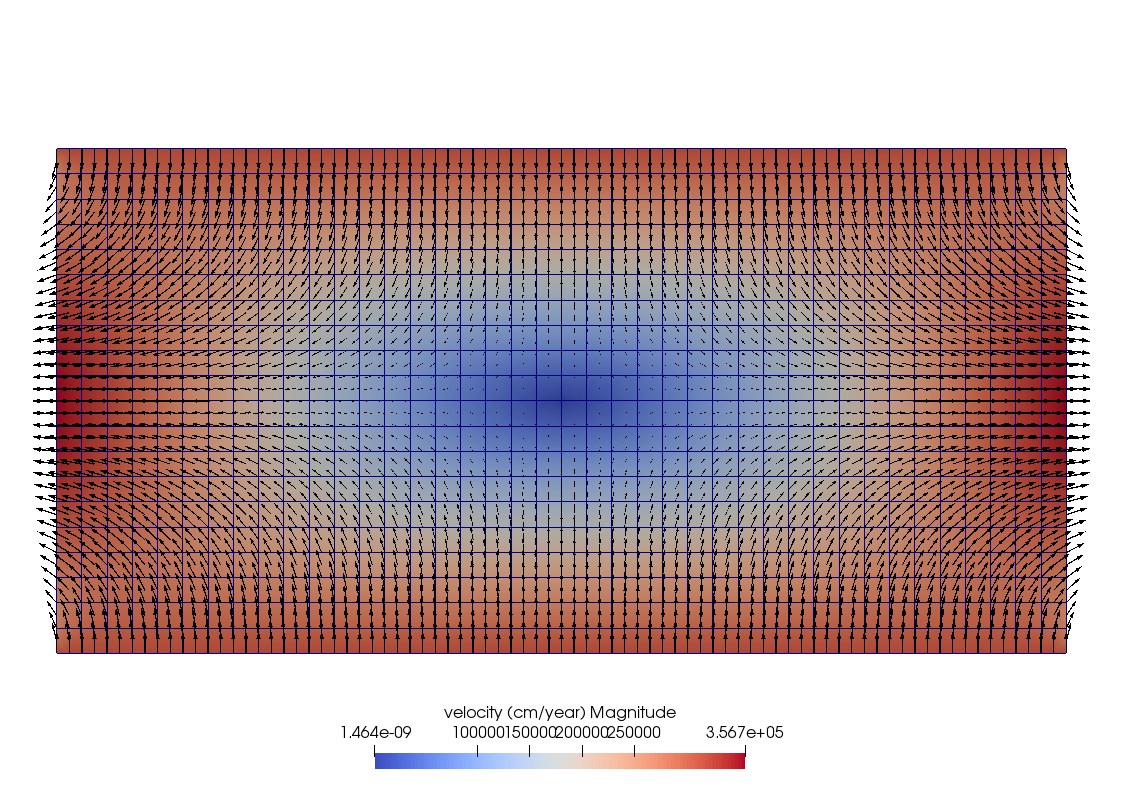
\includegraphics[width=6cm]{python_codes/fieldstone_129/results/experiment5/setup}
\end{center}




